% Options for packages loaded elsewhere
% Options for packages loaded elsewhere
\PassOptionsToPackage{unicode}{hyperref}
\PassOptionsToPackage{hyphens}{url}
%
\documentclass[
  11pt,
  letterpaper,
]{book}
\usepackage{xcolor}
\usepackage[a4paper]{geometry}
\usepackage{amsmath,amssymb}
\setcounter{secnumdepth}{5}
\usepackage{iftex}
\ifPDFTeX
  \usepackage[T1]{fontenc}
  \usepackage[utf8]{inputenc}
  \usepackage{textcomp} % provide euro and other symbols
\else % if luatex or xetex
  \usepackage{unicode-math} % this also loads fontspec
  \defaultfontfeatures{Scale=MatchLowercase}
  \defaultfontfeatures[\rmfamily]{Ligatures=TeX,Scale=1}
\fi
\usepackage{lmodern}
\ifPDFTeX\else
  % xetex/luatex font selection
\fi
% Use upquote if available, for straight quotes in verbatim environments
\IfFileExists{upquote.sty}{\usepackage{upquote}}{}
\IfFileExists{microtype.sty}{% use microtype if available
  \usepackage[]{microtype}
  \UseMicrotypeSet[protrusion]{basicmath} % disable protrusion for tt fonts
}{}
\makeatletter
\@ifundefined{KOMAClassName}{% if non-KOMA class
  \IfFileExists{parskip.sty}{%
    \usepackage{parskip}
  }{% else
    \setlength{\parindent}{0pt}
    \setlength{\parskip}{6pt plus 2pt minus 1pt}}
}{% if KOMA class
  \KOMAoptions{parskip=half}}
\makeatother
% Make \paragraph and \subparagraph free-standing
\makeatletter
\ifx\paragraph\undefined\else
  \let\oldparagraph\paragraph
  \renewcommand{\paragraph}{
    \@ifstar
      \xxxParagraphStar
      \xxxParagraphNoStar
  }
  \newcommand{\xxxParagraphStar}[1]{\oldparagraph*{#1}\mbox{}}
  \newcommand{\xxxParagraphNoStar}[1]{\oldparagraph{#1}\mbox{}}
\fi
\ifx\subparagraph\undefined\else
  \let\oldsubparagraph\subparagraph
  \renewcommand{\subparagraph}{
    \@ifstar
      \xxxSubParagraphStar
      \xxxSubParagraphNoStar
  }
  \newcommand{\xxxSubParagraphStar}[1]{\oldsubparagraph*{#1}\mbox{}}
  \newcommand{\xxxSubParagraphNoStar}[1]{\oldsubparagraph{#1}\mbox{}}
\fi
\makeatother

\usepackage{color}
\usepackage{fancyvrb}
\newcommand{\VerbBar}{|}
\newcommand{\VERB}{\Verb[commandchars=\\\{\}]}
\DefineVerbatimEnvironment{Highlighting}{Verbatim}{commandchars=\\\{\}}
% Add ',fontsize=\small' for more characters per line
\usepackage{framed}
\definecolor{shadecolor}{RGB}{241,243,245}
\newenvironment{Shaded}{\begin{snugshade}}{\end{snugshade}}
\newcommand{\AlertTok}[1]{\textcolor[rgb]{0.68,0.00,0.00}{#1}}
\newcommand{\AnnotationTok}[1]{\textcolor[rgb]{0.37,0.37,0.37}{#1}}
\newcommand{\AttributeTok}[1]{\textcolor[rgb]{0.40,0.45,0.13}{#1}}
\newcommand{\BaseNTok}[1]{\textcolor[rgb]{0.68,0.00,0.00}{#1}}
\newcommand{\BuiltInTok}[1]{\textcolor[rgb]{0.00,0.23,0.31}{#1}}
\newcommand{\CharTok}[1]{\textcolor[rgb]{0.13,0.47,0.30}{#1}}
\newcommand{\CommentTok}[1]{\textcolor[rgb]{0.37,0.37,0.37}{#1}}
\newcommand{\CommentVarTok}[1]{\textcolor[rgb]{0.37,0.37,0.37}{\textit{#1}}}
\newcommand{\ConstantTok}[1]{\textcolor[rgb]{0.56,0.35,0.01}{#1}}
\newcommand{\ControlFlowTok}[1]{\textcolor[rgb]{0.00,0.23,0.31}{\textbf{#1}}}
\newcommand{\DataTypeTok}[1]{\textcolor[rgb]{0.68,0.00,0.00}{#1}}
\newcommand{\DecValTok}[1]{\textcolor[rgb]{0.68,0.00,0.00}{#1}}
\newcommand{\DocumentationTok}[1]{\textcolor[rgb]{0.37,0.37,0.37}{\textit{#1}}}
\newcommand{\ErrorTok}[1]{\textcolor[rgb]{0.68,0.00,0.00}{#1}}
\newcommand{\ExtensionTok}[1]{\textcolor[rgb]{0.00,0.23,0.31}{#1}}
\newcommand{\FloatTok}[1]{\textcolor[rgb]{0.68,0.00,0.00}{#1}}
\newcommand{\FunctionTok}[1]{\textcolor[rgb]{0.28,0.35,0.67}{#1}}
\newcommand{\ImportTok}[1]{\textcolor[rgb]{0.00,0.46,0.62}{#1}}
\newcommand{\InformationTok}[1]{\textcolor[rgb]{0.37,0.37,0.37}{#1}}
\newcommand{\KeywordTok}[1]{\textcolor[rgb]{0.00,0.23,0.31}{\textbf{#1}}}
\newcommand{\NormalTok}[1]{\textcolor[rgb]{0.00,0.23,0.31}{#1}}
\newcommand{\OperatorTok}[1]{\textcolor[rgb]{0.37,0.37,0.37}{#1}}
\newcommand{\OtherTok}[1]{\textcolor[rgb]{0.00,0.23,0.31}{#1}}
\newcommand{\PreprocessorTok}[1]{\textcolor[rgb]{0.68,0.00,0.00}{#1}}
\newcommand{\RegionMarkerTok}[1]{\textcolor[rgb]{0.00,0.23,0.31}{#1}}
\newcommand{\SpecialCharTok}[1]{\textcolor[rgb]{0.37,0.37,0.37}{#1}}
\newcommand{\SpecialStringTok}[1]{\textcolor[rgb]{0.13,0.47,0.30}{#1}}
\newcommand{\StringTok}[1]{\textcolor[rgb]{0.13,0.47,0.30}{#1}}
\newcommand{\VariableTok}[1]{\textcolor[rgb]{0.07,0.07,0.07}{#1}}
\newcommand{\VerbatimStringTok}[1]{\textcolor[rgb]{0.13,0.47,0.30}{#1}}
\newcommand{\WarningTok}[1]{\textcolor[rgb]{0.37,0.37,0.37}{\textit{#1}}}

\usepackage{longtable,booktabs,array}
\usepackage{calc} % for calculating minipage widths
% Correct order of tables after \paragraph or \subparagraph
\usepackage{etoolbox}
\makeatletter
\patchcmd\longtable{\par}{\if@noskipsec\mbox{}\fi\par}{}{}
\makeatother
% Allow footnotes in longtable head/foot
\IfFileExists{footnotehyper.sty}{\usepackage{footnotehyper}}{\usepackage{footnote}}
\makesavenoteenv{longtable}
\usepackage{graphicx}
\makeatletter
\newsavebox\pandoc@box
\newcommand*\pandocbounded[1]{% scales image to fit in text height/width
  \sbox\pandoc@box{#1}%
  \Gscale@div\@tempa{\textheight}{\dimexpr\ht\pandoc@box+\dp\pandoc@box\relax}%
  \Gscale@div\@tempb{\linewidth}{\wd\pandoc@box}%
  \ifdim\@tempb\p@<\@tempa\p@\let\@tempa\@tempb\fi% select the smaller of both
  \ifdim\@tempa\p@<\p@\scalebox{\@tempa}{\usebox\pandoc@box}%
  \else\usebox{\pandoc@box}%
  \fi%
}
% Set default figure placement to htbp
\def\fps@figure{htbp}
\makeatother


% definitions for citeproc citations
\NewDocumentCommand\citeproctext{}{}
\NewDocumentCommand\citeproc{mm}{%
  \begingroup\def\citeproctext{#2}\cite{#1}\endgroup}
\makeatletter
 % allow citations to break across lines
 \let\@cite@ofmt\@firstofone
 % avoid brackets around text for \cite:
 \def\@biblabel#1{}
 \def\@cite#1#2{{#1\if@tempswa , #2\fi}}
\makeatother
\newlength{\cslhangindent}
\setlength{\cslhangindent}{1.5em}
\newlength{\csllabelwidth}
\setlength{\csllabelwidth}{3em}
\newenvironment{CSLReferences}[2] % #1 hanging-indent, #2 entry-spacing
 {\begin{list}{}{%
  \setlength{\itemindent}{0pt}
  \setlength{\leftmargin}{0pt}
  \setlength{\parsep}{0pt}
  % turn on hanging indent if param 1 is 1
  \ifodd #1
   \setlength{\leftmargin}{\cslhangindent}
   \setlength{\itemindent}{-1\cslhangindent}
  \fi
  % set entry spacing
  \setlength{\itemsep}{#2\baselineskip}}}
 {\end{list}}
\usepackage{calc}
\newcommand{\CSLBlock}[1]{\hfill\break\parbox[t]{\linewidth}{\strut\ignorespaces#1\strut}}
\newcommand{\CSLLeftMargin}[1]{\parbox[t]{\csllabelwidth}{\strut#1\strut}}
\newcommand{\CSLRightInline}[1]{\parbox[t]{\linewidth - \csllabelwidth}{\strut#1\strut}}
\newcommand{\CSLIndent}[1]{\hspace{\cslhangindent}#1}



\setlength{\emergencystretch}{3em} % prevent overfull lines

\providecommand{\tightlist}{%
  \setlength{\itemsep}{0pt}\setlength{\parskip}{0pt}}



 


\makeatletter
\@ifpackageloaded{bookmark}{}{\usepackage{bookmark}}
\makeatother
\makeatletter
\@ifpackageloaded{caption}{}{\usepackage{caption}}
\AtBeginDocument{%
\ifdefined\contentsname
  \renewcommand*\contentsname{Table of contents}
\else
  \newcommand\contentsname{Table of contents}
\fi
\ifdefined\listfigurename
  \renewcommand*\listfigurename{List of Figures}
\else
  \newcommand\listfigurename{List of Figures}
\fi
\ifdefined\listtablename
  \renewcommand*\listtablename{List of Tables}
\else
  \newcommand\listtablename{List of Tables}
\fi
\ifdefined\figurename
  \renewcommand*\figurename{Figure}
\else
  \newcommand\figurename{Figure}
\fi
\ifdefined\tablename
  \renewcommand*\tablename{Table}
\else
  \newcommand\tablename{Table}
\fi
}
\@ifpackageloaded{float}{}{\usepackage{float}}
\floatstyle{ruled}
\@ifundefined{c@chapter}{\newfloat{codelisting}{h}{lop}}{\newfloat{codelisting}{h}{lop}[chapter]}
\floatname{codelisting}{Listing}
\newcommand*\listoflistings{\listof{codelisting}{List of Listings}}
\makeatother
\makeatletter
\makeatother
\makeatletter
\@ifpackageloaded{caption}{}{\usepackage{caption}}
\@ifpackageloaded{subcaption}{}{\usepackage{subcaption}}
\makeatother
\usepackage{bookmark}
\IfFileExists{xurl.sty}{\usepackage{xurl}}{} % add URL line breaks if available
\urlstyle{same}
\hypersetup{
  pdftitle={Open Geoinformatics},
  pdfauthor={Lakshmi Kantakumar},
  hidelinks,
  pdfcreator={LaTeX via pandoc}}


\title{Open Geoinformatics}
\author{Lakshmi Kantakumar}
\date{2026-03-06}
\begin{document}
\frontmatter
\maketitle

\renewcommand*\contentsname{Table of contents}
{
\setcounter{tocdepth}{1}
\tableofcontents
}

\mainmatter
\bookmarksetup{startatroot}

\chapter*{Preface}\label{preface}
\addcontentsline{toc}{chapter}{Preface}

\markboth{Preface}{Preface}

The discipline of Geoinformatics stands at the intersection of
geography, information technology, and earth sciences, providing
powerful tools for spatial data acquisition, analysis, and
decision-making. Its applications span diverse fields such as
environmental management, urban and regional planning, disaster risk
reduction, natural resource monitoring, and governance, reflecting its
growing significance in both academia and industry (Goodchild, 2007; Li,
Dragicevic, \& Veenendaal, 2020).

This lecture note, titled Open Geoinformatics is being prepared as a
comprehensive introductory resource for students, researchers, and
practitioners seeking to build a foundation in geospatial science and
technology. A special emphasis is placed on Free and Open-Source
Software (FOSS) tools and datasets, ensuring that the knowledge imparted
is not only theoretically rigorous but also practically accessible
without licensing restrictions.

The content presents essential concepts of Geographic Information
Systems (GIS), Remote Sensing (RS), Global Navigation Satellite Systems
(GNSS), Spatial Databases, and WebGIS, with a balanced focus on theory
and practice. The structure is designed to support stepwise
learning---beginning with fundamentals and gradually progressing toward
advanced applications and integration of geospatial technologies.

In particular, this work acknowledges the invaluable role of FOSS
geospatial platforms and libraries---including QGIS (QGIS Development
Team, 2024), SAGA GIS (Conrad et al., 2008), PostGIS (PostGIS Project
Steering Committee, 2023), GeoServer (GeoServer Development Team, 2024),
and GDAL/OGR (GDAL/OGR contributors, 2023). These tools, along with
contributions from numerous other open-source projects, not only provide
world-class functionality but also embody the spirit of collaborative
knowledge-building and open science.

The compilation draws upon established literature and best practices in
the field, while also incorporating open-source software environments,
community-driven innovations, and contemporary applications to make the
learning process relevant in today's context. It is hoped that this work
will not only serve as a guide for academic study but also inspire
further exploration, research, and innovation in the open geospatial
domain.

I gratefully acknowledge the contributions of scholars, researchers, and
the global FOSS community whose works form the intellectual and
technical foundation of this discipline. Any inadvertent omission of
citation is unintentional, and suggestions for improvement and inclusion
of additional references are warmly welcomed.

\bookmarksetup{startatroot}

\chapter*{Acknowledgements}\label{acknowledgements}
\addcontentsline{toc}{chapter}{Acknowledgements}

\markboth{Acknowledgements}{Acknowledgements}

This work on \textbf{\emph{Open Geoinformatics is still in progress}},
and at this stage I am sincerely acknowledging the encouragement and
support I am receiving.

I am especially grateful to Shri. Guddanti Varuna Kumar, Additional
Surveyor General, NIGST, who is continuously encouraging me. I am also
thankful to Shri. Mahesh R., Deputy Surveyor General, NIGST, Shri.
Pankaj Mishra, Deputy Surveyor General, NIGST, and Shri. D.K. Singh,
Deputy Surveyor General, NIGST, who are guiding and motivating me during
the development of this work.

A very special acknowledgement is due to Shri. Yoga Chandra P.A.,
Superintending Surveyor, NIGST, whose constant encouragement and belief
in my potential are being a true driving force. His support is pushing
me beyond my limits and giving me the confidence to keep progressing
with dedication. I am grateful to Shri. Pankaj Singh Kalam,
Superintending Surveyor, NIGST, for his encouragement.

I am also sincerely appreciating the support of Shri. Anand Saga M.,
Officer Surveyor, NIGST, Shri. P. Mohan Krishna, Officer Surveyor,
NIGST, Shri. Basava Raju, Surveyor, NIGST, and Shri. M.V. Subbarao,
D/Man Div-I, NIGST to shape this book.

I am further acknowledging all others at NIGST who are supporting and
encouraging me in this ongoing effort, as their involvement is proving
invaluable while I continue working towards the completion of this work.

Finally, I am expressing my deepest gratitude to my family members,
whose patience, understanding, and unwavering support are being my true
foundation and strength as I move forward in this journey.

\part{Module 1: Free and Open-Source Software (FOSS) Geoinformatics}

\chapter{Introduction to
Geoinformatics}\label{introduction-to-geoinformatics}

\section{What is Geoinformatics?}\label{what-is-geoinformatics}

Have you ever used Google Maps to find the quickest route, checked the
weather forecast, or tracked a delivery package? These everyday
conveniences are possible because of a field known as
\textbf{Geoinformatics}.

In simple terms, Geoinformatics is the science and technology concerned
with the collection, storage, processing, analysis, and visualization of
spatial (location-based) data. It seeks to answer fundamental questions
such as

\begin{itemize}
\tightlist
\item
  \emph{Where is something located?}
\item
  \emph{What is happening there?} and
\item
  \emph{How does it relate to its surroundings?}
\end{itemize}

Geoinformatics is an interdisciplinary field that integrates
\textbf{Geographic Information Systems (GIS), Remote Sensing (RS),
Global Navigation Satellite Systems (GNSS), cartography, digital image
processing, spatial databases, GeoAI and web mapping} into a unified
workflow. It supports the \textbf{acquisition, management, analysis,
visualization, and sharing} of spatial information for decision-making.

\section{Importance of
Geoinformatics}\label{importance-of-geoinformatics}

The world today is highly dynamic. Cities are expanding, natural
resources are being depleted, and environmental challenges such as
climate change and natural disasters are becoming more frequent. To
manage these issues effectively, accurate spatial data and strong
analytical capabilities are essential.

Geoinformatics provides this ability and supports a wide range of
activities such as:

\begin{itemize}
\tightlist
\item
  Planning and decision-making for urban growth, infrastructure, and
  governance\\
\item
  Environmental monitoring of forests, water bodies, and pollution\\
\item
  Disaster management through early warning systems and risk
  assessments\\
\item
  Efficient transport and navigation systems\\
\item
  Sustainable agriculture and food security through precision farming
\end{itemize}

In essence, Geoinformatics transforms spatial data into actionable
knowledge for informed decision-making.

\subsection{Key capabilities of
Geoinformatics}\label{key-capabilities-of-geoinformatics}

\begin{itemize}
\tightlist
\item
  \textbf{Data acquisition}: satellite/aerial remote sensing, GNSS
  positioning, ground surveys, and IoT sensors.\\
\item
  \textbf{Data management}: spatial databases, metadata, and spatial
  data infrastructures (SDIs).\\
\item
  \textbf{Spatial analysis and modeling}: image processing, terrain
  analysis, network analysis, and environmental modeling.\\
\item
  \textbf{Visualization and communication}: maps, dashboards, 3D/4D
  views, and web platforms.
\end{itemize}

\subsection{Workflow overview}\label{workflow-overview}

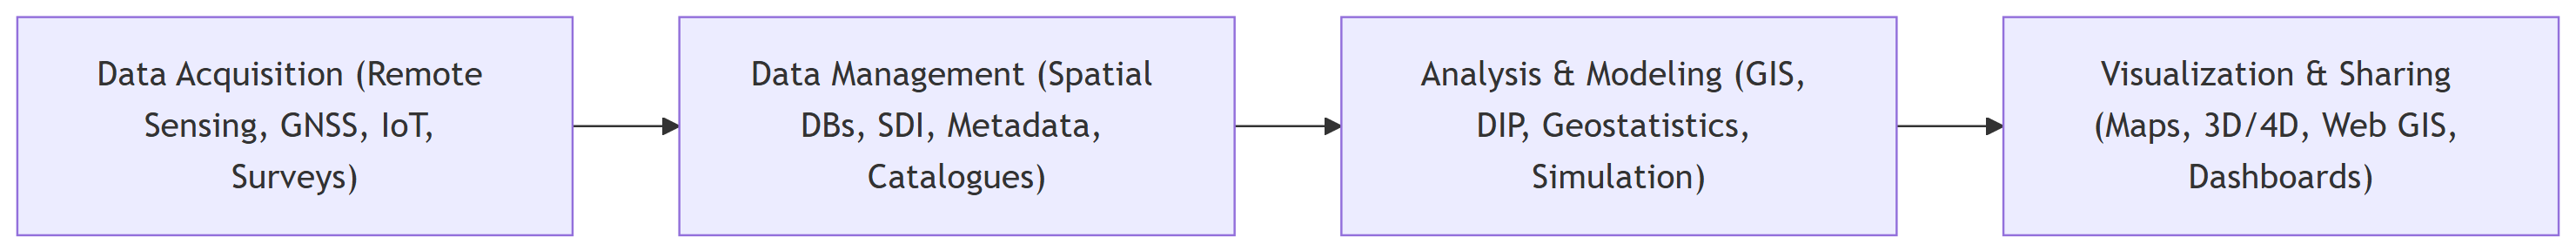
\includegraphics[width=12.56in,height=1.23in]{chapters/module_1/introduction_files/figure-latex/mermaid-figure-1.png}

\section{Components of
Geoinformatics}\label{components-of-geoinformatics}

Geoinformatics is based on several interconnected technologies,
including:

\begin{itemize}
\tightlist
\item
  \textbf{Remote Sensing (RS):} The collection of Earth data using
  satellites, drones, and aircraft\\
\item
  \textbf{Geographic Information Systems (GIS):} Computer-based systems
  for storing, analyzing, and displaying spatial data\\
\item
  \textbf{Global Navigation Satellite Systems (GNSS):} Technologies such
  as GPS that provide accurate positioning and navigation services\\
\item
  \textbf{Cartography and Visualization:} Methods for representing data
  through maps, 3D models, and interactive systems\\
\item
  \textbf{Spatial Data Infrastructure (SDI):} Frameworks and
  institutions that support data sharing and accessibility\\
\item
  \textbf{Digital Image Processing (DIP):} Techniques for enhancing,
  classifying, and analyzing remotely sensed imagery and other raster
  data to extract meaningful information.
\item
  \textbf{Web Mapping and Web GIS:} Internet-based tools and services
  that deliver, analyze, and integrate spatial information through
  interactive web platforms and APIs.
\item
  \textbf{GeoAI (Geospatial Artificial Intelligence):} Application of
  artificial intelligence, machine learning, and deep learning
  techniques to spatial data for tasks such as image classification,
  predictive modeling, feature extraction, and automated
  decision-making.
\end{itemize}

\begin{figure}

\centering{

\includegraphics[width=0.7\linewidth,height=\textheight,keepaspectratio]{chapters/module_1/figures/geoinformatics.png}

}

\caption{\label{fig-geoinformatics}\emph{Geoinformatics}}

\end{figure}%

\section{Evolution of Geoinformatics}\label{evolution-of-geoinformatics}

The development of Geoinformatics reflects humanity's evolving
relationship with spatial data. In the past, geographic information was
measured and represented manually through surveys and cartographic
techniques. With the introduction of aerial photography and later
satellite imaging, data collection became faster and more accurate.

The digital revolution of the 20th century enabled computer-based
mapping and Geographic Information Systems (GIS), which greatly expanded
analytical possibilities. Today, cloud computing, artificial
intelligence, and big data are transforming Geoinformatics into a
real-time and dynamic discipline.

\section{Applications of
Geoinformatics}\label{applications-of-geoinformatics}

Geoinformatics has diverse applications across sectors. Some key
examples include:

\begin{itemize}
\tightlist
\item
  \textbf{Disaster Management:} Flood mapping, earthquake impact
  assessment, and forest fire monitoring\\
\item
  \textbf{Environmental Studies:} Climate change monitoring, pollution
  tracking, and conservation planning\\
\item
  \textbf{Urban and Regional Planning:} Smart city development,
  infrastructure planning, and land-use analysis\\
\item
  \textbf{Agriculture:} Precision farming, soil health assessment, and
  crop yield prediction\\
\item
  \textbf{Transportation and Logistics:} Route optimization, vehicle
  tracking, and supply chain management\\
\item
  \textbf{Defense and Security:} Terrain analysis, border surveillance,
  and communication systems
\end{itemize}

\section{The Open Dimension}\label{the-open-dimension}

An essential characteristic of modern Geoinformatics is the increasing
role of \textbf{open-source software and open data}. Unlike proprietary
systems, which often involve high licensing costs and limited
flexibility, open platforms are freely available, shaped by global
communities, and can be tailored to diverse applications.

Well-known tools such as \textbf{QGIS}, \textbf{GRASS GIS},
\textbf{PostGIS}, \textbf{GeoServer}, and \textbf{SAGA GIS}, along with
community-driven projects like \textbf{OpenStreetMap (OSM)}, offer
robust and accessible options for spatial analysis, data handling, and
online data sharing. Through these resources, Geoinformatics has become
more \textbf{democratic, inclusive, and participatory}. More than just
technological solutions, they embody a broader philosophy of openness,
cooperation, and shared responsibility in using spatial knowledge to
address global challenges.

\section{Future of Geoinformatics}\label{future-of-geoinformatics}

Geoinformatics is continuously evolving with emerging technologies.
Future directions include:

\begin{itemize}
\tightlist
\item
  Artificial Intelligence and Machine Learning for automated analysis of
  satellite imagery\\
\item
  Internet of Things (IoT) for integrating ground-based sensors with
  geospatial systems\\
\item
  Digital Twins for creating dynamic, real-time models of cities and
  natural systems\\
\item
  Drone-based mapping for high-resolution, flexible data collection\\
\item
  Citizen science and open data initiatives that encourage public
  participation in data generation
\end{itemize}

In the future, Geoinformatics will not only describe what is happening
but also predict future scenarios and guide decisions for sustainable
development.

\section{Conclusion}\label{conclusion}

Geoinformatics is more than the study of maps. It is a modern discipline
that integrates technology with geography to provide solutions for
real-world challenges. From disaster management to urban planning and
environmental protection, its applications are vast and significant.

With the rise of open-source software and open data initiatives,
Geoinformatics has become more accessible and collaborative than ever
before. This inclusive approach is shaping the way we understand and
manage our planet.

Thus, \textbf{Open Geoinformatics} represents not only the science of
spatial data but also the philosophy of openness, collaboration, and
shared knowledge for a sustainable future. The next chapter explores
this openness further by introducing \textbf{Free and Open-Source
Software (FOSS)}, which forms the foundation of modern geospatial
practice.

\chapter{Free and Open-Source Software}\label{sec-intro}

\section{FOSS}\label{foss}

Free and Open-Source Software (FOSS) refers to software released under a
license that grants users essential freedoms to run it for any purpose,
examine how it works, adapt it to their needs, and share it, whether in
its original form or with modifications, without limitations or fees.
The term \textbf{FOSS} blends two closely related ideas: \textbf{free
software}, which focuses on user rights and collaborative ownership, and
\textbf{open-source software}, which stresses transparency and
community-driven development.

\begin{figure}

\centering{

\includegraphics[width=0.7\linewidth,height=\textheight,keepaspectratio]{chapters/module_1/figures/foss.png}

}

\caption{\label{fig-foss}\emph{Free and Open-Source Software}}

\end{figure}%

\section{Free Software ≠ Open Source}\label{free-software-open-source}

Richard Stallman, founder of the Free Software Movement, points out that
while \textbf{free software} and \textbf{open source} often describe the
same kind of programs, they are based on different ideas.

\begin{itemize}
\tightlist
\item
  \textbf{Free software} is about \emph{freedom} making sure people
  control the software they use.\\
\item
  \textbf{Open source} is more about \emph{practical benefits} like
  better quality and faster development, without focusing much on the
  moral side\\
  (\href{https://www.gnu.org}{gnu.org}).
\end{itemize}

\begin{center}\rule{0.5\linewidth}{0.5pt}\end{center}

\section{The Four Freedoms of Free
Software}\label{the-four-freedoms-of-free-software}

``Free'' here means \emph{freedom}, not zero cost. Free software means
you can:

\begin{figure}

\centering{

\includegraphics[width=0.7\linewidth,height=\textheight,keepaspectratio]{chapters/module_1/figures/Pillars_of_FS.png}

}

\caption{\label{fig-FS}\emph{The Four Freedoms of Free Software}}

\end{figure}%

\begin{itemize}
\tightlist
\item
  \textbf{Freedom 0} : Use the program however you want.\\
\item
  \textbf{Freedom 1} : Look at the code and change it to fit your
  needs.\\
\item
  \textbf{Freedom 2} : Give copies to anyone.\\
\item
  \textbf{Freedom 3} : Share your improved versions with others.
\end{itemize}

(Source:
\href{https://en.wikipedia.org/wiki/The_Free_Software_Definition}{Wikipedia})

\begin{center}\rule{0.5\linewidth}{0.5pt}\end{center}

\section{A Short History}\label{a-short-history}

\begin{itemize}
\tightlist
\item
  \textbf{1983} : The Free Software Movement began with the GNU Project
  and a license (GPL) that made sure these freedoms were protected
  (\href{https://en.wikipedia.org/wiki/GNU_Project}{Wikipedia}).\\
\item
  \textbf{1998} : Some in the community started calling it ``open
  source'' to make the idea sound more appealing to businesses. This
  approach often skipped talking about the moral side of software
  freedom (\href{https://www.gnu.org}{gnu.org}).
\end{itemize}

\begin{center}\rule{0.5\linewidth}{0.5pt}\end{center}

\section{The Open Source Definition
(OSD)}\label{the-open-source-definition-osd}

The \textbf{Open Source Definition (OSD)}, managed by the
\href{https://opensource.org}{Open Source Initiative (OSI)}, explains
what counts as open-source software. Created in \textbf{2006} and last
updated in \textbf{February 2024}, it lists \textbf{ten rules} that go
beyond just sharing the code. Open Source software means you can:

\begin{itemize}
\tightlist
\item
  \textbf{Free sharing} : no fees or restrictions.\\
\item
  \textbf{Source code included} : in a form you can read and edit.\\
\item
  \textbf{Changes allowed} : you can make and share new versions.\\
\item
  \textbf{Works on any tech} : no limits based on platform or hardware.
\end{itemize}

These rules make sure open-source software stays free to \textbf{use},
\textbf{change}, and \textbf{share}, giving a clear and trusted meaning
for developers, communities, and businesses.

\begin{figure}

\centering{

\includegraphics[width=0.7\linewidth,height=\textheight,keepaspectratio]{chapters/module_1/figures/Pillars_of_OSS.png}

}

\caption{\label{fig-FS}\emph{The ten rules of Open Source Software}}

\end{figure}%

\begin{center}\rule{0.5\linewidth}{0.5pt}\end{center}

\section{Different Ways of Thinking}\label{different-ways-of-thinking}

While both groups create similar kinds of software, they make choices
differently:

\begin{itemize}
\tightlist
\item
  \textbf{Open source thinking:} ``Is this the best tool for the job?''
  may use closed, paid software if it's more convenient.\\
\item
  \textbf{Free software thinking:} ``Does this respect my freedom?''
  avoids closed software even if it's technically better.
\end{itemize}

\begin{center}\rule{0.5\linewidth}{0.5pt}\end{center}

\section{Comparison: Free Software vs Open
Source}\label{comparison-free-software-vs-open-source}

\begin{longtable}[]{@{}
  >{\raggedright\arraybackslash}p{(\linewidth - 4\tabcolsep) * \real{0.1583}}
  >{\raggedright\arraybackslash}p{(\linewidth - 4\tabcolsep) * \real{0.4317}}
  >{\raggedright\arraybackslash}p{(\linewidth - 4\tabcolsep) * \real{0.4101}}@{}}
\caption{Free Software vs Open Source
comparison}\label{tbl-comparison}\tabularnewline
\toprule\noalign{}
\begin{minipage}[b]{\linewidth}\raggedright
Aspect
\end{minipage} & \begin{minipage}[b]{\linewidth}\raggedright
Free Software
\end{minipage} & \begin{minipage}[b]{\linewidth}\raggedright
Open Source Software
\end{minipage} \\
\midrule\noalign{}
\endfirsthead
\toprule\noalign{}
\begin{minipage}[b]{\linewidth}\raggedright
Aspect
\end{minipage} & \begin{minipage}[b]{\linewidth}\raggedright
Free Software
\end{minipage} & \begin{minipage}[b]{\linewidth}\raggedright
Open Source Software
\end{minipage} \\
\midrule\noalign{}
\endhead
\bottomrule\noalign{}
\endlastfoot
\textbf{Emphasis} & Focuses on \textbf{freedom} (user rights) & Focuses
on \textbf{development model} and practical benefits \\
\textbf{Founded by} & Richard Stallman (Free Software Foundation - FSF)
& Eric Raymond \& Bruce Perens (Open Source Initiative - OSI) \\
\textbf{Core Idea} & Users should control the software they use & Open
code leads to better, more reliable software \\
\textbf{Terminology} & ``Free'' means freedom, not price (``free as in
freedom'') & ``Open Source'' avoids the ambiguity of the word
``free'' \\
\textbf{Ethical Standpoint} & A \textbf{moral and social movement} & A
\textbf{development methodology} \\
\textbf{Licensing} & Requires \textbf{copyleft licenses} (e.g., GPL) to
protect freedom & Accepts \textbf{permissive licenses} (e.g., MIT, BSD,
Apache) \\
\textbf{Goal} & Empower users with freedoms to use, study, modify, share
& Promote wider adoption of open development practices \\
\textbf{Tone \& Messaging} & Often ideological & Often pragmatic and
business-friendly \\
\end{longtable}

\begin{center}\rule{0.5\linewidth}{0.5pt}\end{center}

\section{Conclusion}\label{conclusion-1}

Free and Open-Source Software represents more than just a different way
to build and share code, it reflects two complementary philosophies that
have shaped modern software culture. While the Free Software movement
champions user freedoms as a moral imperative, the Open Source approach
emphasizes collaboration, transparency, and practical benefits.
Together, they have fostered a global ecosystem where knowledge is
openly shared, innovation thrives, and communities,from hobbyists to
governments can create, adapt, and distribute technology without
restrictive barriers.

The next chapter explores the framework that makes this openness
possible by introducing \textbf{FOSS licenses}, which define the rights
and responsibilities that guide how software can be used, modified, and
shared.

\chapter{Free and Open-Source Software (FOSS)
licenses}\label{sec-licenses}

\section{Introduction}\label{introduction}

\textbf{Free and Open-Source Software (FOSS) licenses} are rules that
explain how you can use, change, and share a piece of software. They
make sure the promises of FOSS, like seeing the code, improving it, and
sharing it; are protected by law.

Think of them as:

\begin{itemize}
\tightlist
\item
  \textbf{A shield} protecting your rights as a user.
\item
  \textbf{A guide} showing how people can work together and reuse code.
\end{itemize}

Not all FOSS licenses are the same. Some, called copyleft licenses,
require any changed versions to stay open. Others, called permissive
licenses, give you more freedom to reuse the code, even in closed-source
projects.

\begin{center}\rule{0.5\linewidth}{0.5pt}\end{center}

\section{Copyleft Licenses (Restrictive / Strong
Share-Alike)}\label{copyleft-licenses-restrictive-strong-share-alike}

These licenses require that derivative works and redistributions also
remain under the same license.

\begin{longtable}[]{@{}
  >{\raggedright\arraybackslash}p{(\linewidth - 2\tabcolsep) * \real{0.2804}}
  >{\raggedright\arraybackslash}p{(\linewidth - 2\tabcolsep) * \real{0.7196}}@{}}
\caption{Common Copyleft Licenses}\label{tbl-cllic}\tabularnewline
\toprule\noalign{}
\begin{minipage}[b]{\linewidth}\raggedright
License Name
\end{minipage} & \begin{minipage}[b]{\linewidth}\raggedright
Key Features
\end{minipage} \\
\midrule\noalign{}
\endfirsthead
\toprule\noalign{}
\begin{minipage}[b]{\linewidth}\raggedright
License Name
\end{minipage} & \begin{minipage}[b]{\linewidth}\raggedright
Key Features
\end{minipage} \\
\midrule\noalign{}
\endhead
\bottomrule\noalign{}
\endlastfoot
GNU General Public License (GPL) & Must release modified code under same
license; widely used in FSF projects \\
GNU Lesser GPL (LGPL) & Allows linking with proprietary code (for
libraries); milder than GPL \\
AGPL (Affero GPL) & Extends GPL to network services must release source
even when software is only accessed over a network \\
EUPL & European Union Public License similar to GPL, legally compliant
in EU jurisdictions \\
\end{longtable}

\textbf{The Goal of Copyleft Licenses} is to protect user freedoms by
enforcing openness downstream (\emph{strong reciprocity}).

\begin{center}\rule{0.5\linewidth}{0.5pt}\end{center}

\section{Permissive Licenses (Non-Restrictive / Minimal
Requirements)}\label{permissive-licenses-non-restrictive-minimal-requirements}

These licenses allow reuse in both open and proprietary projects, with
minimal conditions.

\begin{longtable}[]{@{}
  >{\raggedright\arraybackslash}p{(\linewidth - 2\tabcolsep) * \real{0.2871}}
  >{\raggedright\arraybackslash}p{(\linewidth - 2\tabcolsep) * \real{0.7129}}@{}}
\caption{Common Permissive Licenses}\label{tbl-perlic}\tabularnewline
\toprule\noalign{}
\begin{minipage}[b]{\linewidth}\raggedright
License Name
\end{minipage} & \begin{minipage}[b]{\linewidth}\raggedright
Key Features
\end{minipage} \\
\midrule\noalign{}
\endfirsthead
\toprule\noalign{}
\begin{minipage}[b]{\linewidth}\raggedright
License Name
\end{minipage} & \begin{minipage}[b]{\linewidth}\raggedright
Key Features
\end{minipage} \\
\midrule\noalign{}
\endhead
\bottomrule\noalign{}
\endlastfoot
MIT License & Simple, Very permissive; Just requires attribution \\
Apache License 2.0 & Allows patent use; More corporate-friendly than
MIT \\
BSD Licenses (2-clause, 3-clause) & Minimal restrictions; Used in BSD OS
family \\
ISC License & Even simpler than MIT; No warranties, Attribution
required \\
\end{longtable}

\textbf{The Goal of Permissive Licenses} is to maximize freedom to use
and integrate, including in closed-source projects.

\begin{center}\rule{0.5\linewidth}{0.5pt}\end{center}

\section{Copyleft vs Permissive licenses - Key
Differences}\label{copyleft-vs-permissive-licenses---key-differences}

In general, \textbf{Copyleft licenses} protect the \emph{freedom of the
code}. \textbf{Permissive licenses} prioritize \emph{freedom for
developers and businesses}.

\begin{longtable}[]{@{}
  >{\raggedright\arraybackslash}p{(\linewidth - 4\tabcolsep) * \real{0.3529}}
  >{\raggedright\arraybackslash}p{(\linewidth - 4\tabcolsep) * \real{0.3137}}
  >{\raggedright\arraybackslash}p{(\linewidth - 4\tabcolsep) * \real{0.3333}}@{}}
\caption{Copyleft vs Permissive licenses key Differences
comparison}\label{tbl-liccomp}\tabularnewline
\toprule\noalign{}
\begin{minipage}[b]{\linewidth}\raggedright
Feature
\end{minipage} & \begin{minipage}[b]{\linewidth}\raggedright
Copyleft (GPL)
\end{minipage} & \begin{minipage}[b]{\linewidth}\raggedright
Permissive (MIT/Apache)
\end{minipage} \\
\midrule\noalign{}
\endfirsthead
\toprule\noalign{}
\begin{minipage}[b]{\linewidth}\raggedright
Feature
\end{minipage} & \begin{minipage}[b]{\linewidth}\raggedright
Copyleft (GPL)
\end{minipage} & \begin{minipage}[b]{\linewidth}\raggedright
Permissive (MIT/Apache)
\end{minipage} \\
\midrule\noalign{}
\endhead
\bottomrule\noalign{}
\endlastfoot
Requires same license for derivatives & Yes & No \\
Allows proprietary use & No & Yes \\
Popular with & Free Software movement & Businesses, startups \\
\end{longtable}

\section{Conclusion}\label{conclusion-2}

FOSS licenses form the legal backbone of the open-source ecosystem,
ensuring that the freedoms to use, study, modify, and share software are
upheld. While \textbf{copyleft licenses} safeguard these freedoms by
requiring derivatives to remain open, \textbf{permissive licenses} focus
on flexibility, enabling integration into both open and proprietary
projects. Understanding these license types is essential for developers,
organizations, and policymakers to choose the right balance between
protecting openness and encouraging broader adoption. In essence, the
right license not only defines how software is shared but also shapes
the culture of collaboration and innovation in the FOSS community.

Building on this foundation, the next chapter introduces \textbf{FOSS
GIS}, where these licensing principles meet the world of geospatial
technologies, enabling powerful, accessible, and collaborative tools for
spatial analysis and decision-making.

\chapter{Introduction to FOSS
Geoinformatics}\label{introduction-to-foss-geoinformatics}

\section{What is FOSS
Geoinformatics?}\label{what-is-foss-geoinformatics}

\emph{Free and Open Source Software (FOSS) Geoinformatics} includes
applications and libraries whose \textbf{source code is openly
available} for use, study, modification, and redistribution under open
licenses. FOSS spans the entire spatial workflow:

\begin{itemize}
\tightlist
\item
  \textbf{GIS} for mapping and spatial analysis.\\
\item
  \textbf{Remote sensing \& digital image processing} for Earth
  observation data.\\
\item
  \textbf{GNSS} for precise positioning and navigation.\\
\item
  \textbf{Web GIS \& spatial databases} for publishing and
  interoperability.\\
\item
  \textbf{Visualization} for communication and decision support.
\end{itemize}

\section{Why FOSS Geoinformatics
Matters}\label{why-foss-geoinformatics-matters}

\begin{itemize}
\tightlist
\item
  \textbf{Affordable access}: lowers entry barriers for education,
  community use, NGOs, and startups.\\
\item
  \textbf{Community-driven development}: global collaboration supports
  continuous improvement.\\
\item
  \textbf{Adaptability}: tools can be customized for local workflows and
  languages.\\
\item
  \textbf{Transparency}: open code enables verification of methods and
  security.\\
\item
  \textbf{Capacity building}: encourages learning and experimentation.\\
\item
  \textbf{Interoperability}: open standards (e.g., OGC/ISO) enable
  integration across platforms.\\
\item
  \textbf{Platform flexibility}: commonly available for Linux, Windows,
  and macOS.\\
\item
  \textbf{Integration across domains}: unifies GIS, RS, GNSS, databases,
  and the web.
\end{itemize}

\section{Examples of Popular FOSS Geoinformatics
Tools}\label{examples-of-popular-foss-geoinformatics-tools}

The FOSS geoinformatics ecosystem includes desktop analysis, satellite
data processing, web mapping, database management, and GNSS processing.

\begin{longtable}[]{@{}
  >{\raggedright\arraybackslash}p{(\linewidth - 6\tabcolsep) * \real{0.2500}}
  >{\raggedright\arraybackslash}p{(\linewidth - 6\tabcolsep) * \real{0.2500}}
  >{\raggedright\arraybackslash}p{(\linewidth - 6\tabcolsep) * \real{0.2500}}
  >{\raggedright\arraybackslash}p{(\linewidth - 6\tabcolsep) * \real{0.2500}}@{}}
\caption{Examples of Popular FOSS Geoinformatics
Tools}\label{tbl-fossgeo}\tabularnewline
\toprule\noalign{}
\begin{minipage}[b]{\linewidth}\raggedright
\textbf{Software}
\end{minipage} & \begin{minipage}[b]{\linewidth}\raggedright
\textbf{Domain}
\end{minipage} & \begin{minipage}[b]{\linewidth}\raggedright
\textbf{Description}
\end{minipage} & \begin{minipage}[b]{\linewidth}\raggedright
\textbf{License Type}
\end{minipage} \\
\midrule\noalign{}
\endfirsthead
\toprule\noalign{}
\begin{minipage}[b]{\linewidth}\raggedright
\textbf{Software}
\end{minipage} & \begin{minipage}[b]{\linewidth}\raggedright
\textbf{Domain}
\end{minipage} & \begin{minipage}[b]{\linewidth}\raggedright
\textbf{Description}
\end{minipage} & \begin{minipage}[b]{\linewidth}\raggedright
\textbf{License Type}
\end{minipage} \\
\midrule\noalign{}
\endhead
\bottomrule\noalign{}
\endlastfoot
\textbf{QGIS} & GIS & Desktop GIS with a rich plugin ecosystem for
mapping and analysis. & GNU GPL v2 \\
\textbf{GRASS GIS} & GIS/RS/DIP & Advanced raster--vector processing,
image classification, and modeling. & GNU GPL v2 \\
\textbf{SAGA GIS} & GIS/Environmental & Raster analysis, geomorphometry,
and terrain modeling. & GNU GPL v2 \\
\textbf{WhiteboxTools} & DIP/Modeling & LiDAR tools, hydrology, and
raster processing with Python/R bindings. & MIT \\
\textbf{ESA SNAP} & Remote Sensing & Processing of Sentinel and other EO
missions. & GNU GPL v3 \\
\textbf{Orfeo Toolbox (OTB)} & Remote Sensing & High-performance image
analysis and change detection (C++/Python). & Apache 2.0 \\
\textbf{PDAL} & Point Clouds & Ingests, filters, and transforms
LiDAR/point cloud data. & BSD \\
\textbf{PostGIS} & Spatial DB & Spatial extension for PostgreSQL;
advanced spatial queries and indexing. & GNU GPL v2 \\
\textbf{SpatiaLite} & Spatial DB & SQLite with spatial capabilities for
lightweight deployments. & MPL/GPL/LGPL \\
\textbf{GeoServer} & Web GIS & Publishes data via OGC services
(WMS/WFS/WCS/WPS). & GNU GPL v2 \\
\textbf{MapServer} & Web GIS & High-performance map rendering server. &
MIT \\
\textbf{OpenLayers} & Web GIS & JavaScript library for interactive web
maps. & BSD \\
\textbf{Leaflet} & Web GIS & Lightweight web-mapping JavaScript library.
& BSD \\
\textbf{OpenStreetMap} & Open Data & Global, community-curated basemap
and POI dataset. & ODbL \\
\textbf{RTKLIB} & GNSS & Precise GNSS processing (PPP/RTK) for GPS,
GLONASS, Galileo, etc. & BSD \\
\textbf{GPSTk (GPS Toolkit)} & GNSS & Libraries and apps for GNSS
positioning and research (C++). & GNU LGPL \\
\textbf{goGPS} & GNSS & GNSS processing and sensor fusion (MATLAB/Python
variants). & GPL \\
\textbf{GNSS-SDR} & GNSS & Software-defined receiver framework; raw data
to position. & GPL v3 \\
\end{longtable}

\section{Importance of Open-Source Data \& Software in NGP
2022}\label{importance-of-open-source-data-software-in-ngp-2022}

The \textbf{National Geospatial Policy (NGP) 2022} encourages
\textbf{open standards, open data, and open-source platforms}. This
direction promotes accessibility, interoperability, and reuse across
agencies, academia, industry, and communities.

By promoting FOSS Geoinformatics:

\begin{itemize}
\tightlist
\item
  \textbf{Communities} can use spatial data for local planning and risk
  reduction.\\
\item
  \textbf{Educational institutions} can train students without licensing
  restrictions.\\
\item
  \textbf{Startups and NGOs} can develop cost-effective geospatial
  services.
\end{itemize}

This approach supports a \textbf{self-reliant, transparent, and
future-ready geospatial ecosystem}, reduces vendor dependence, and
strengthens collaboration.

\section{Conclusion}\label{conclusion-3}

FOSS Geoinformatics is reshaping how spatial data are \textbf{collected,
processed, analyzed, and communicated}. Open tools such as \textbf{QGIS,
GRASS GIS, OTB, SNAP, PostGIS, GeoServer}, and open GNSS stacks like
\textbf{RTKLIB, GPSTk, goGPS, and GNSS-SDR} enable integrated and
interoperable workflows. Communities worldwide can now contribute to and
benefit from shared spatial knowledge, empowering students, researchers,
governments, and industries to solve real-world problems.

However, true collaboration requires more than just open tools and data.
Different systems must follow common rules to share and understand
information effectively. This is where \textbf{open standards} become
essential, providing the universal language that makes geospatial
technologies interoperable. The next chapter introduces these open
standards.

\chapter{Introduction to Open
Standards}\label{introduction-to-open-standards}

\section{Introduction}\label{introduction-1}

Geospatial data today powers everything from navigation apps to climate
research. For this information to be useful, it must be
\textbf{interoperable}; that is, capable of moving between different
platforms, software, and organizations without compatibility issues. The
\textbf{Open Geospatial Consortium (OGC)} develops \emph{open standards}
that make this possible, ensuring a common ``language'' for geospatial
data exchange and processing (OGC, 2025).

\begin{center}\rule{0.5\linewidth}{0.5pt}\end{center}

\section{What are Open Standards?}\label{what-are-open-standards}

\textbf{Open Standards} are publicly available specifications that
define how software systems should exchange data and communicate.\\
They allow interoperability, prevent vendor lock-in, and encourage
innovation by ensuring that multiple tools can share and process the
same data.

\emph{Example}: A flood map generated in ArcGIS can be visualized in
QGIS or Google Earth if shared using an OGC standard such as
\textbf{WMS} or \textbf{KML}.

\begin{center}\rule{0.5\linewidth}{0.5pt}\end{center}

\section{Key Characteristics of Open
Standards}\label{key-characteristics-of-open-standards}

\begin{itemize}
\tightlist
\item
  \textbf{Publicly available}: Anyone can access and implement them.\\
\item
  \textbf{Interoperable}: Allow different systems to work together
  seamlessly.\\
\item
  \textbf{Non-proprietary}: Not controlled by a single vendor.\\
\item
  \textbf{Consensus-driven}: Developed collaboratively by communities of
  experts.\\
\item
  \textbf{Widely adopted}: Used across industries, governments, and
  academia.\\
\item
  \textbf{Future-oriented}: Designed to evolve with new technological
  trends.
\end{itemize}

\begin{center}\rule{0.5\linewidth}{0.5pt}\end{center}

\section{OGC Standards Landscape}\label{ogc-standards-landscape}

OGC standards can be broadly grouped into three categories (OGC, 2025):

\subsection{Modern OGC APIs (REST/JSON)}\label{modern-ogc-apis-restjson}

Developed for the modern web, these standards use REST principles and
lightweight formats like \textbf{JSON} (JavaScript Object Notation).
They are developer-friendly and cloud-ready.

\begin{itemize}
\tightlist
\item
  \textbf{OGC API -- Features}: Access vector features.\\
\item
  \textbf{OGC API -- Maps}: Retrieve maps dynamically.\\
\item
  \textbf{OGC API -- Tiles}: Fetch tiled map layers.\\
\item
  \textbf{OGC SensorThings API}: Manage Internet of Things (IoT) sensor
  data.
\end{itemize}

\subsection{Legacy Web Services
(XML-based)}\label{legacy-web-services-xml-based}

Earlier standards relied on XML (eXtensible Markup Language) and remote
procedure calls. They remain widely used in geospatial applications.

\begin{itemize}
\tightlist
\item
  \textbf{WMS (Web Map Service)}: Provides map images.\\
\item
  \textbf{WFS (Web Feature Service)}: Provides vector features with
  attributes.\\
\item
  \textbf{WCS (Web Coverage Service)}: Provides raster or coverage
  data.\\
\item
  \textbf{WPS (Web Processing Service)}: Runs geospatial processing
  tasks online.
\end{itemize}

\subsection{Data Models and Encodings}\label{data-models-and-encodings}

These specify how geospatial data is structured and exchanged.

\begin{itemize}
\tightlist
\item
  \textbf{GML (Geography Markup Language)}: XML-based representation of
  features.\\
\item
  \textbf{KML (Keyhole Markup Language)}: XML-based, widely used for map
  visualization.\\
\item
  \textbf{GeoJSON}: Lightweight JSON format, popular in web mapping.
\end{itemize}

\begin{center}\rule{0.5\linewidth}{0.5pt}\end{center}

\section{TL;DR Summary Table}\label{tldr-summary-table}

The OGC standards ecosystem is broad and sometimes overwhelming. To make
things easier, the following table provides a \emph{``Too Long; Didn't
Read (TL;DR) overview''}, summarizing the major categories of standards,
their examples, and their key use cases at a glance.

\begin{longtable}[]{@{}
  >{\raggedright\arraybackslash}p{(\linewidth - 4\tabcolsep) * \real{0.1905}}
  >{\raggedright\arraybackslash}p{(\linewidth - 4\tabcolsep) * \real{0.4286}}
  >{\raggedright\arraybackslash}p{(\linewidth - 4\tabcolsep) * \real{0.3810}}@{}}
\caption{Summary Table of Major Categories of
Standards}\label{tbl-standards}\tabularnewline
\toprule\noalign{}
\begin{minipage}[b]{\linewidth}\raggedright
\textbf{Category}
\end{minipage} & \begin{minipage}[b]{\linewidth}\raggedright
\textbf{Examples}
\end{minipage} & \begin{minipage}[b]{\linewidth}\raggedright
\textbf{Notes}
\end{minipage} \\
\midrule\noalign{}
\endfirsthead
\toprule\noalign{}
\begin{minipage}[b]{\linewidth}\raggedright
\textbf{Category}
\end{minipage} & \begin{minipage}[b]{\linewidth}\raggedright
\textbf{Examples}
\end{minipage} & \begin{minipage}[b]{\linewidth}\raggedright
\textbf{Notes}
\end{minipage} \\
\midrule\noalign{}
\endhead
\bottomrule\noalign{}
\endlastfoot
\textbf{Modern APIs} & OGC API -- Features, Maps, Tiles, SensorThings &
REST/JSON, lightweight, cloud-friendly \\
\textbf{Legacy Web Services} & WMS, WFS, WCS, WPS & XML-based, still
widely used in many systems \\
\textbf{Data Encodings} & GML, KML, GeoJSON & Define how data is
structured and exchanged \\
\end{longtable}

\begin{center}\rule{0.5\linewidth}{0.5pt}\end{center}

\section{Deep Dive into Key
Standards}\label{deep-dive-into-key-standards}

Understanding the standards at a deeper level is useful for
practitioners and students who want to see how they are applied in
practice.\\
While the landscape provides categories, each standard has a specific
purpose and set of strengths. Below are some of the most widely
recognized OGC standards.

\begin{itemize}
\tightlist
\item
  \textbf{API -- Features}: A modern RESTful replacement for WFS.\\
\item
  \textbf{WMS}: Suited for sharing static map images.\\
\item
  \textbf{WFS}: Useful when raw vector data is needed for analysis.\\
\item
  \textbf{WCS}: Designed for raster data like satellite imagery and
  DEMs.\\
\item
  \textbf{KML}: Popular for sharing points, routes, and polygons in
  Google Earth.\\
\item
  \textbf{GML}: A more complex but powerful format for rich geospatial
  datasets.
\end{itemize}

\begin{center}\rule{0.5\linewidth}{0.5pt}\end{center}

\section{Standards Lifecycle}\label{standards-lifecycle}

OGC follows a community-driven process for developing new standards
(OGC, 2025):

\begin{enumerate}
\def\labelenumi{\arabic{enumi}.}
\tightlist
\item
  \textbf{Problem Identification} → Recognize a gap or need.\\
\item
  \textbf{Draft Specification} → Experts write a proposed solution.\\
\item
  \textbf{Testing \& Pilots} → Validate the draft in real-world
  projects.\\
\item
  \textbf{Consensus \& Voting} → Members review and approve.\\
\item
  \textbf{Publication} → The standard becomes publicly available.\\
\item
  \textbf{Maintenance} → Continuous updates for new requirements.
\end{enumerate}

\begin{center}\rule{0.5\linewidth}{0.5pt}\end{center}

\section{Real-World Impact}\label{real-world-impact}

Geospatial data only becomes truly powerful when it can be shared and
understood across organizations, sectors, and borders. This is where OGC
standards show their real value.\\
They \textbf{transform abstract specifications into practical tools}
that enable disaster response, scientific research, urban planning, and
even daily navigation apps.\\
The following mini case studies illustrate how OGC standards make a
tangible difference in solving real-world problems and improving
decision-making at both national and global levels.

\subsection{Disaster Management and Emergency
Response}\label{disaster-management-and-emergency-response}

\begin{itemize}
\tightlist
\item
  \textbf{Challenge:} During floods, wildfires, or earthquakes, response
  agencies need fast, accurate geospatial data from multiple sources.\\
\item
  \textbf{OGC Solution:} Standards like \textbf{Web Map Service (WMS)}
  and \textbf{Web Feature Service (WFS)} allow data from satellites,
  drones, and ground sensors to be instantly shared across platforms.\\
\item
  \textbf{Impact:} Agencies in different countries can visualize the
  same map layers, monitor real-time conditions, and coordinate rescue
  operations more effectively.
\end{itemize}

\subsection{Urban Planning and Smart
Cities}\label{urban-planning-and-smart-cities}

\begin{itemize}
\tightlist
\item
  \textbf{Challenge:} Modern cities deal with issues like traffic
  congestion, zoning, and infrastructure development. Multiple agencies
  often use different software systems, making collaboration
  difficult.\\
\item
  \textbf{OGC Solution:} \textbf{CityGML} and \textbf{IndoorGML} enable
  the creation of interoperable 3D city models and building layouts.\\
\item
  \textbf{Impact:} Urban planners can integrate building, transport, and
  environmental data into a common model, leading to better planning
  decisions, optimized public transport, and improved disaster
  preparedness.
\end{itemize}

\subsection{Environmental Monitoring and Climate
Change}\label{environmental-monitoring-and-climate-change}

\begin{itemize}
\tightlist
\item
  \textbf{Challenge:} Monitoring deforestation, air pollution, or
  climate change requires combining datasets from satellites, sensors,
  and models.\\
\item
  \textbf{OGC Solution:} \textbf{Web Coverage Service (WCS)} and
  \textbf{Sensor Observation Service (SOS)} enable sharing of raster
  datasets and real-time sensor feeds.\\
\item
  \textbf{Impact:} Scientists and policymakers gain access to
  consistent, comparable data across nations, improving environmental
  research and enabling international agreements on climate action.
\end{itemize}

\subsection{Agriculture and Food
Security}\label{agriculture-and-food-security}

\begin{itemize}
\tightlist
\item
  \textbf{Challenge:} Farmers and governments require timely geospatial
  data on soil, rainfall, and crop health to improve yields and food
  security.\\
\item
  \textbf{OGC Solution:} \textbf{OGC APIs} and \textbf{Geography Markup
  Language (GML)} allow integration of satellite imagery, IoT sensors,
  and predictive models.\\
\item
  \textbf{Impact:} Farmers can receive precision agriculture advisories,
  and governments can manage food supply chains more efficiently,
  reducing hunger risks.
\end{itemize}

\subsection{Everyday Applications -- Navigation and Location
Services}\label{everyday-applications-navigation-and-location-services}

\begin{itemize}
\tightlist
\item
  \textbf{Challenge:} Billions of users rely on maps for navigation,
  ride-sharing, and logistics, often without realizing the complexity of
  data integration behind the scenes.\\
\item
  \textbf{OGC Solution:} Standards like \textbf{KML (Keyhole Markup
  Language)} power Google Earth and other map-based applications.\\
\item
  \textbf{Impact:} Users benefit from accurate, up-to-date geospatial
  information, while companies can build interoperable services that
  work seamlessly worldwide.
\end{itemize}

\begin{center}\rule{0.5\linewidth}{0.5pt}\end{center}

\section{Future Directions}\label{future-directions}

The geospatial standards landscape continues to evolve as new
technologies, data formats, and user needs emerge. OGC is actively
shaping this evolution to ensure that standards remain relevant,
lightweight, and capable of supporting modern geospatial applications.

The future of OGC standards can be described through several \textbf{key
trends and priority areas}, a few of which are listed below.

\subsection{Transition from XML to JSON/RESTful
APIs}\label{transition-from-xml-to-jsonrestful-apis}

\begin{itemize}
\tightlist
\item
  \textbf{Past Approach:} Early OGC standards such as WMS, WFS, and WCS
  were primarily built on \textbf{XML-based protocols} (e.g., GML).
  While powerful, they can be verbose and complex, making them less
  developer-friendly.\\
\item
  \textbf{Emerging Approach:} Modern \textbf{OGC APIs} (like API --
  Features, API -- Tiles, API -- Processes) are based on \textbf{REST
  principles and JSON encoding}.\\
\item
  \textbf{Benefits:}

  \begin{itemize}
  \tightlist
  \item
    Easier integration with modern web and mobile applications\\
  \item
    Lightweight data exchange\\
  \item
    Better compatibility with cloud-native architectures\\
  \item
    Lower barriers for developers outside traditional GIS domains
  \end{itemize}
\end{itemize}

\subsection{Cloud-Native and Big Data
Integration}\label{cloud-native-and-big-data-integration}

\begin{itemize}
\tightlist
\item
  As datasets grow in size (e.g., petabytes of satellite imagery), OGC
  is working on standards that support \textbf{cloud-native data
  storage} (e.g., Cloud Optimized GeoTIFFs, SpatioTemporal Asset Catalog
  -- STAC).\\
\item
  These enable \textbf{on-demand access} to only the portion of data
  needed, improving performance and reducing costs for analytics at
  scale.
\end{itemize}

\subsection{Real-Time and IoT-Enabled Geospatial
Data}\label{real-time-and-iot-enabled-geospatial-data}

\begin{itemize}
\tightlist
\item
  The growth of \textbf{Internet of Things (IoT)} devices (e.g.,
  sensors, smart vehicles, drones) requires standards that can handle
  \textbf{continuous, real-time data streams}.\\
\item
  OGC standards like the \textbf{SensorThings API} are designed for
  this, supporting smart cities, environmental monitoring, and disaster
  response.
\end{itemize}

\subsection{AI/ML and Analytics
Integration}\label{aiml-and-analytics-integration}

\begin{itemize}
\tightlist
\item
  Future standards will increasingly need to accommodate \textbf{machine
  learning and AI pipelines}.\\
\item
  Interoperability is being extended beyond raw data sharing to include
  \textbf{standardized access to geospatial analytics services}, helping
  to integrate AI models directly into workflows.
\end{itemize}

\subsection{Cross-Domain
Interoperability}\label{cross-domain-interoperability}

\begin{itemize}
\tightlist
\item
  Geospatial data is no longer isolated. It connects with domains like
  \textbf{healthcare, climate science, agriculture, defense, and
  transportation}.\\
\item
  OGC's \textbf{Domain Working Groups (DWGs)} are focusing on ensuring
  geospatial standards integrate seamlessly with other international
  standards (ISO, W3C, IEEE).
\end{itemize}

\subsection{The Role of the OGC Reference Model
(ORM)}\label{the-role-of-the-ogc-reference-model-orm}

\begin{itemize}
\tightlist
\item
  The \textbf{OGC Reference Model (ORM)} continues to provide a
  \textbf{conceptual framework} for understanding how all standards fit
  together.\\
\item
  It helps guide the transition from \textbf{legacy services} to
  \textbf{modern APIs}, ensuring that innovation does not break existing
  systems while providing a roadmap for future adoption.
\end{itemize}

In summary, the future of OGC standards is moving toward
\textbf{lighter, faster, cloud-friendly, and developer-oriented
solutions} while maintaining the core principle of \textbf{global
interoperability}. Together, these emerging directions ensure that OGC
standards remain a cornerstone for achieving interoperability, enabling
seamless data sharing, and supporting innovative applications across
diverse domains. This evolution guarantees that geospatial information
will continue to be a critical enabler of innovation in the digital era.

\begin{center}\rule{0.5\linewidth}{0.5pt}\end{center}

\section{Conclusion}\label{conclusion-4}

OGC standards serve as the \textbf{universal language of geospatial
information}, enabling seamless data sharing across platforms and
fostering collaboration between governments, industry, and academia.
They have evolved from early XML-based services such as WMS and WFS to
modern, lightweight RESTful APIs that better align with today's web and
cloud ecosystems. Through this evolution, OGC standards have
consistently made geospatial data more accessible, interoperable, and
impactful; helping societies address global challenges such as disaster
management, climate monitoring, sustainable development, and smart city
planning.

\begin{center}\rule{0.5\linewidth}{0.5pt}\end{center}

\part{Module 2: GIS}

\chapter{Introduction to GIS}\label{introduction-to-gis}

\section{What is GIS?}\label{what-is-gis}

A Geographic Information System (GIS) is a computer-based framework that
allows us to work with information that has a spatial or geographic
component. In simple terms, GIS links \textbf{``what'' data is about}
with \textbf{``where'' it is located on Earth}. This combination makes
it possible to explore patterns, detect relationships, and make informed
decisions.

\subsection{Definition of GIS}\label{definition-of-gis}

A Geographic Information System (GIS) is a framework that supports the
collection, management, analysis, and visualization of spatial and
non-spatial data. It integrates hardware, software, data, people, and
methods to efficiently handle geographically referenced information
{[}Albrecht (2007); Wilson \& Fotheringham (2008){]}. By linking data to
locations on Earth, GIS allows users to capture, store, manipulate, and
display information that supports decision-making in fields such as
urban planning, environmental management, agriculture, transportation,
and disaster response {[}Yang, Wong, Miao, \& Yang (2011){]}.

\section{Components of GIS}\label{components-of-gis}

A GIS is composed of several interconnected components that work
together:

\begin{itemize}
\tightlist
\item
  \textbf{Hardware}: Computing systems with adequate processing power,
  memory, storage, and input/output devices.
\item
  \textbf{Software}: GIS applications and operating systems that provide
  tools for data analysis, management, and visualization.
\item
  \textbf{Data}: Spatial data (geographic features), attribute data
  (descriptive information), and metadata (documentation about quality
  and origin).
\item
  \textbf{People}: Users and professionals who design, implement, and
  apply GIS solutions.
\item
  \textbf{Methods}: Procedures and workflows that ensure data
  acquisition, analysis, validation, and presentation follow consistent
  standards {[}Brimicombe (2010){]}.
\end{itemize}

These components interact continuously. Without reliable data, advanced
software, or skilled users, the system would not function effectively.

\section{Why GIS is Important?}\label{why-gis-is-important}

GIS has become essential because it improves efficiency and accuracy in
working with geographic information. Its benefits include:

\begin{itemize}
\tightlist
\item
  Handling large datasets more effectively than manual methods.
\item
  Supporting complex spatial queries and analyses.
\item
  Allowing integration of diverse datasets from multiple sources.
\item
  Reducing redundancy by linking spatial and attribute information.
\item
  Providing powerful visualization and communication tools {[}Yang et
  al. (2011){]}.
\end{itemize}

\section{Functions of GIS}\label{functions-of-gis}

The main functions of GIS are closely connected, with each step
supporting the next:

\begin{itemize}
\item
  \textbf{Data capture}: Collecting information through digitization,
  scanning, remote sensing, and GNSS.
\item
  \textbf{Data storage and management}: Organizing vector and raster
  models, with indexing and metadata to support retrieval and
  integration.

  \begin{itemize}
  \tightlist
  \item
    \textbf{Vector}: Represents discrete objects such as roads and
    parcels.
  \item
    \textbf{Raster}: Represents continuous surfaces such as elevation
    and temperature.
  \end{itemize}
\item
  \textbf{Querying}: Retrieving data by spatial location or attribute
  values.
\item
  \textbf{Analysis}: Using tools such as buffering, overlay,
  interpolation, and terrain modeling.
\item
  \textbf{Visualization}: Producing maps, graphs, dashboards, and 3D
  visualizations.
\item
  \textbf{Output and communication}: Delivering results in reports, web
  maps, or decision-support systems {[}Campbell \& Wynne (2011){]}.
\end{itemize}

\section{GIS Workflow}\label{gis-workflow}

A typical GIS workflow progresses through several connected stages:

\subsection{Data Acquisition}\label{data-acquisition}

This stage involves collecting raw spatial and attribute data. Sources
include ground surveys, GPS, aerial photography, satellite imagery, and
existing databases. Reliable data acquisition ensures that subsequent
steps are based on accurate representations of real-world phenomena.

\subsection{Data Validation}\label{data-validation}

Validation checks the accuracy and consistency of the acquired data.
Errors such as missing values, spatial mismatches, and attribute
inconsistencies are identified and corrected. This step improves the
quality of data and builds confidence for further analysis.

\subsection{Data Management}\label{data-management}

Validated data is organized into databases or spatial infrastructures.
Processes such as georeferencing, projection transformations, and
indexing make the data usable. Effective management ensures the data can
be retrieved and updated when needed.

\subsection{Data Analysis and
Modeling}\label{data-analysis-and-modeling}

At this stage, GIS tools are applied to derive insights. Analyses may
include overlays, spatial statistics, change detection, and predictive
modeling. This step transforms raw data into meaningful information that
supports planning and decision-making.

\subsection{Visualization and Output}\label{visualization-and-output}

Finally, results are communicated through clear visual formats. These
include thematic maps, 3D views, dashboards, or printed reports.
Effective visualization ensures that technical results are accessible to
both specialists and non-specialists.

\textbf{Workflow Diagram:}

\begin{figure}

\centering{

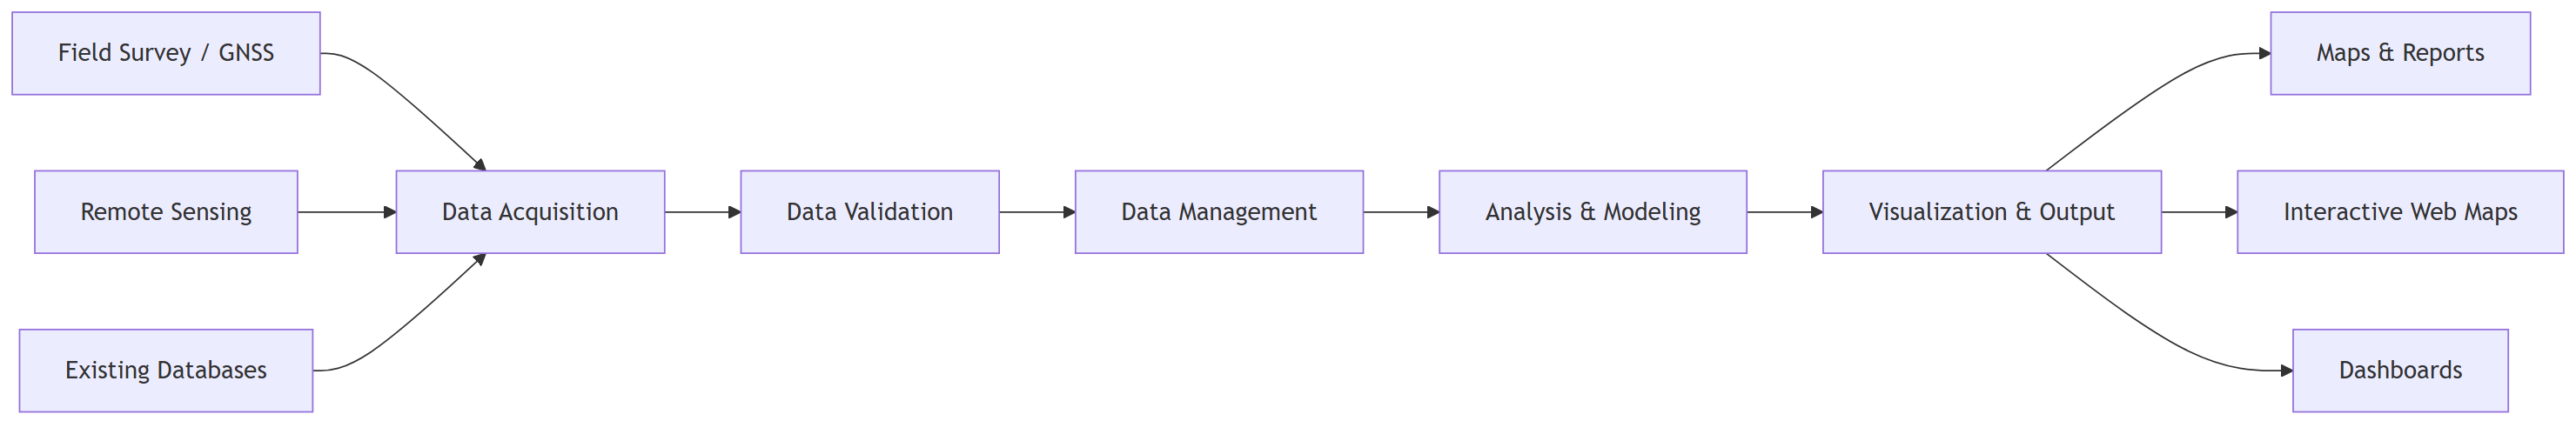
\includegraphics[width=17.58in,height=2.9in]{chapters/module_2/gis-intro_files/figure-latex/mermaid-figure-1.png}

}

\caption{\label{fig-workflow}Typical GIS workflow}

\end{figure}%

\section{Some Standard GIS Softwares}\label{some-standard-gis-softwares}

\begin{longtable}[]{@{}
  >{\raggedright\arraybackslash}p{(\linewidth - 4\tabcolsep) * \real{0.2069}}
  >{\raggedright\arraybackslash}p{(\linewidth - 4\tabcolsep) * \real{0.3276}}
  >{\raggedright\arraybackslash}p{(\linewidth - 4\tabcolsep) * \real{0.4655}}@{}}
\toprule\noalign{}
\begin{minipage}[b]{\linewidth}\raggedright
Software
\end{minipage} & \begin{minipage}[b]{\linewidth}\raggedright
License Type
\end{minipage} & \begin{minipage}[b]{\linewidth}\raggedright
Author/Company
\end{minipage} \\
\midrule\noalign{}
\endhead
\bottomrule\noalign{}
\endlastfoot
\textbf{ArcGIS} & Proprietary & Esri (Environmental Systems Research
Institute) \\
\textbf{QGIS} & Open-source (GPL) & QGIS Development Team
(community-driven) \\
\textbf{GRASS GIS} & Open-source (GPL) & GRASS Development Team
(originally US Army CERL) \\
\textbf{MapInfo Professional} & Proprietary & Pitney Bowes Software
(originally MapInfo Corporation) \\
\textbf{Google Earth Pro} & Freeware (Proprietary) & Google LLC \\
\textbf{ERDAS IMAGINE} & Proprietary & Hexagon Geospatial
(Intergraph/Leica Geosystems) \\
\textbf{ENVI} & Proprietary & Harris Geospatial Solutions (L3Harris
Technologies) \\
\textbf{IDRISI/TerrSet} & Proprietary (Academic License options) & Clark
Labs, Clark University \\
\textbf{PostGIS} & Open-source (GPL) & Refractions Research, now
community-maintained \\
\end{longtable}

\subsection{Open-source vs Proprietary
GIS}\label{open-source-vs-proprietary-gis}

Open-source platforms such as QGIS, GRASS, and PostGIS are
cost-effective, adaptable, and community-supported. They provide
transparency of source code and strong plugin ecosystems, although they
may lack formal support and advanced commercial features.

Proprietary platforms such as ArcGIS, ENVI, and ERDAS IMAGINE are
robust, well-documented, and supported by dedicated companies. However,
they are expensive and less flexible for customization.

\section{Future Trends in GIS}\label{future-trends-in-gis}

The future of GIS is shaped by new technologies:

\begin{itemize}
\tightlist
\item
  \textbf{Web GIS} and \textbf{cloud computing} are making GIS more
  scalable and accessible.
\item
  \textbf{Artificial Intelligence and Machine Learning} support
  predictive analytics and pattern recognition.
\item
  \textbf{Mobile GIS} allows real-time data collection in the field.
\item
  \textbf{Big data integration} strengthens spatial analysis of complex
  and large-scale phenomena {[}Wilson \& Fotheringham (2008); Yang et
  al. (2011){]}.
\end{itemize}

\section{Applications of GIS}\label{applications-of-gis}

\begin{itemize}
\item
  \textbf{Urban growth and land-use planning}\\
  GIS helps city planners design sustainable urban spaces by analyzing
  existing land use, population growth, and infrastructure availability.
  It supports zoning decisions, urban renewal projects, and smart city
  initiatives.
\item
  \textbf{Monitoring of natural resources and environment}\\
  GIS is widely used in forestry, water management, soil conservation,
  and biodiversity protection. It allows continuous monitoring of
  ecosystems and helps authorities detect environmental degradation
  early.
\item
  \textbf{Emergency response and disaster risk reduction}\\
  Hazard-prone areas can be mapped with GIS to prepare for disasters
  like floods, cyclones, or earthquakes. During emergencies, it supports
  real-time coordination of evacuation routes, shelters, and relief
  supplies.
\item
  \textbf{Transportation planning and navigation services}\\
  From traffic analysis to public transport route optimization, GIS
  enables efficient mobility planning. It also powers everyday
  navigation apps that millions rely on for real-time directions.
\item
  \textbf{Health studies such as disease mapping}\\
  By mapping the spread of diseases, GIS reveals spatial patterns of
  outbreaks and helps allocate medical resources. It also supports
  vaccination campaigns and long-term healthcare infrastructure
  planning.
\item
  \textbf{Market research and business logistics}\\
  Businesses use GIS for site selection, customer profiling, competitor
  analysis, and logistics optimization. Delivery companies rely on GIS
  to design cost-efficient and timely distribution routes.
\item
  \textbf{Agriculture and precision farming}\\
  Farmers and agricultural agencies apply GIS to monitor soil quality,
  rainfall, crop health, and pest outbreaks. Precision farming uses
  spatial data to apply fertilizers and water efficiently, improving
  productivity while reducing costs.
\item
  \textbf{Climate change studies}\\
  Researchers use GIS to model rising sea levels, shifting vegetation
  zones, glacial retreat, and temperature variations. This helps
  governments plan mitigation and adaptation strategies at both local
  and global scales.
\item
  \textbf{Archaeology and cultural heritage management}\\
  GIS assists archaeologists in locating excavation sites, mapping
  ancient landscapes, and preserving cultural heritage. Museums and
  heritage authorities also use GIS to manage monuments and visitor
  facilities.
\item
  \textbf{Public utilities and infrastructure management}\\
  Utility companies rely on GIS to manage water pipelines, electricity
  networks, and telecommunication lines. It helps detect faults, plan
  maintenance, and ensure efficient service delivery.
\item
  \textbf{Crime analysis and law enforcement}\\
  Police and security agencies use GIS to analyze crime hotspots, study
  spatial patterns of offenses, and optimize patrolling routes. This
  improves public safety and law enforcement efficiency.
\item
  \textbf{Tourism and recreation planning}\\
  Tourism boards and park authorities employ GIS to map attractions,
  hiking trails, and facilities. It also supports eco-tourism by
  balancing visitor access with conservation.
\end{itemize}

\section{Conclusion}\label{conclusion-5}

GIS integrates spatial and non-spatial data to support informed
decision-making in diverse fields such as urban planning, environmental
monitoring, agriculture, and disaster management. Its workflow from
acquisition to visualization ensures that data becomes useful
information. As technology advances, GIS is becoming more accessible,
intelligent, and integrated with other systems.

The next chapter will focus on \textbf{GIS Data}, introducing the
different types of data used in GIS, including vector, raster, and
attribute data, along with their characteristics and applications.

\chapter{Georeferencing}\label{georeferencing}

\section{Concept and Definition of
Georeferencing}\label{concept-and-definition-of-georeferencing}

Georeferencing is the process of assigning real-world geographic
coordinates to spatial data such as scanned maps, aerial photographs,
satellite images, or drone-acquired imagery. It helps create a spatial
relationship between the image's pixels and the geographic location of
the Earth's surface, thus enabling the integration of diverse datasets
with a single reference system (Huisman O., 2009). This technique helps
ensure that spatial data is correctly related to its location on the
Earth's surface, thus being useful for decision-making and spatial
analysis.

Georeferencing is the backbone of a GIS, as all other processes and
functions, such as distance calculation, overlay, or change detection,
depend on it. Without georeferencing, the data will exist independently
in the coordinate space, and it will be impossible to compare and
combine them. For instance, a scanned map of the topographic surface
will be impossible to compare with satellite images or cadastral
boundaries if it is not georeferenced.

\begin{figure}

\centering{

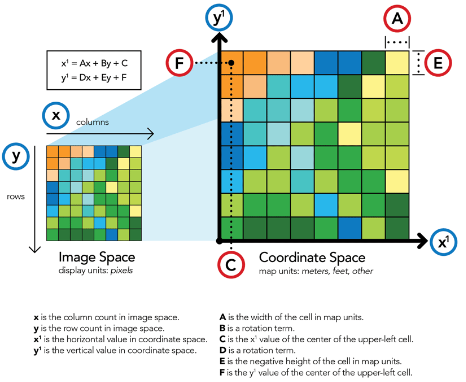
\includegraphics[width=0.7\linewidth,height=\textheight,keepaspectratio]{chapters/module_2/figures/geo_intro.png}

}

\caption{\label{fig-geo}\emph{Diagram showing the relationship between
image coordinates (pixels) and geographic coordinates on Earth (Credit:
\href{https://www.esri.com/about/newsroom/arcuser/understanding-raster-georeferencing}{ESRI})}}

\end{figure}%

In practical terms, georeferencing can be viewed as a transformation
between image coordinate systems (row and column indices) and
Earth-based coordinates (latitude, longitude, or projected coordinates
such as UTM Easting and Northing). The transformation process often
involves identifying a set of known control points, which are used to
compute mathematical relationships between the image and real-world
coordinate systems (Campbell \& Wynne, 2011).

\section{The Need and Importance of
Georeferencing}\label{the-need-and-importance-of-georeferencing}

The accuracy and reliability of the results obtained using a GIS depend
on the quality of the geospatial data alignment with the real world.
Georeferencing is the process of ensuring that the data has a common
spatial reference system, which is essential in integrating different
types of data, such as satellite images, GPS field data, and existing
geospatial data (Wilson \& Fotheringham, 2008). Without georeferencing,
it is possible that results can be inaccurate due to improper data
alignment.

\begin{figure}

\centering{

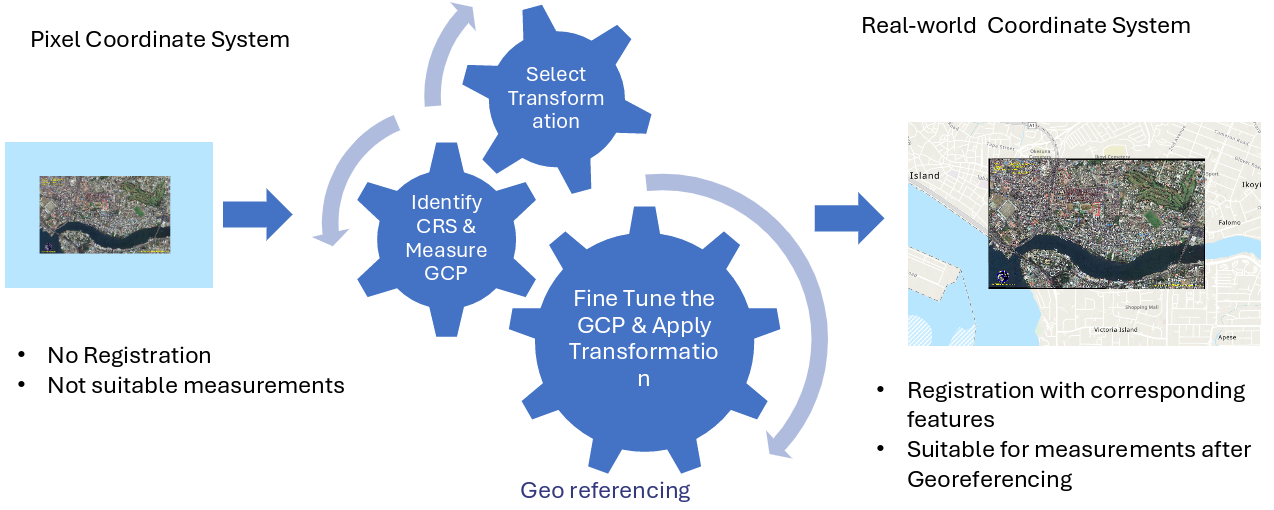
\includegraphics[width=0.7\linewidth,height=\textheight,keepaspectratio]{chapters/module_2/figures/geo_flow.png}

}

\caption{\label{fig-geo}\emph{Process of Georeferencing}}

\end{figure}%

Georeferencing is particularly important since the source data is, in
many instances, based on analog maps developed before the era of digital
cartographic tools. In fact, these maps, which are normally in paper or
soft copy formats, have to be georeferenced in order to conform to the
current standard systems, for example the Universal Transverse Mercator
system based on the World Geodetic System 1984. The technique is not
only vital in the context of national mapping and spatial planning but
also in the integration of historical archives with new data obtained
from satellite and aerial sources. For example, it is possible to study
changes in land cover and urban growth by georeferencing the 1970s
topographic maps with Sentinel-2 satellite images. Without
georeferencing, it would not be possible.

\section{Coordinate Systems and Map
Projections}\label{coordinate-systems-and-map-projections}

A coordinate system is used as a guide for locating the position of
geographic features on the surface of the Earth. Georeferencing involves
the allocation of coordinates to each pixel or feature. Coordinate
systems can be categorized into geographic coordinate systems and
projected coordinate systems (Albrecht, 2007)).

\subsection{Geographic Coordinate
System}\label{geographic-coordinate-system}

The geographic coordinate system (GCS) is defined as the system of
coordinates that uses angular measurements of latitude and longitude to
define positions on the surface of the Earth, modeled as a spheroid or
ellipsoid. The most common geographic datum used worldwide is the World
Geodetic System of 1984 (WGS84). Nevertheless, various nations,
including India, used their own geographic systems, such as the Everest
Datum, based on Everest ellipsoid.

\subsection{Projected Coordinate
System}\label{projected-coordinate-system}

The projected coordinate system (PCS) is defined as the system that
transforms the curved surface of the Earth to a plane using mathematical
formulas. The most common PCS is the Universal Transverse Mercator (UTM)
projection, where the world is divided into 60 zones, each 6° wide in
longitude. India is located within UTM Zones 42N to 47N. The PCS is
mostly used for calculating distances and areas, which cannot be
accurately done using angular measurements used in Geographic Coordinate
System.

\subsection{Relationship between Datum, Projection, and Coordinate
System}\label{relationship-between-datum-projection-and-coordinate-system}

It is important to note that a coordinate system is considered complete
when both datum and projection parameters have been considered.
Inconsistency in datum, such as when data is in National Geodeatic
Reference Frame (NGRF) Datum on WGS84 Elliposid is overlaid on Everest
datum, can cause positional inaccuracies of up to hundreds of meters.
Therefore, it is important to take note of all coordinate references
when georeferencing data.

\section{Ground Control Points (GCPs): Role and
Selection}\label{ground-control-points-gcps-role-and-selection}

Ground Control Points, or GCPs, refer to precise locations that can
easily be identified on the image as well as the actual scene. GCPs play
an important role in the georeferencing process, as they form the basis
for the computation of the transformation parameters that connect the
two coordinate systems, the image coordinates, and the actual scene
coordinates (Richards, 2013). GCPs have an important bearing on the
quality of the georeferencing process.

\begin{figure}

\centering{

\includegraphics[width=0.7\linewidth,height=\textheight,keepaspectratio]{chapters/module_2/figures/geo_geo.png}

}

\caption{\label{fig-geo}\emph{The role of GCP}}

\end{figure}%

\subsection{Characteristics of Good
GCPs}\label{characteristics-of-good-gcps}

\begin{itemize}
\tightlist
\item
  Permanence: The features used as GCP should remain unchanging over
  time, e.g., intersections of roads, corners of buildings, or
  monuments.
\item
  Clarity: The features used as GCP should be easily identifiable both
  on the image and the corresponding map.
\item
  Distribution: The GCPs should be evenly distributed over the image to
  reduce distortion effects.
\item
  Accuracy: The coordinates should be derived from reliable sources,
  e.g., GNSS measurements in the field or official topographic project
  databases.
\end{itemize}

\subsection{Sources of GCPs}\label{sources-of-gcps}

GCPs can be collected from the following sources: - GPS measurements in
the field using GNSS survey techniques for high accuracy. - Existing
datasets that have been previously georeferenced, e.g., existing
topographic maps or orthophotos. - Publicly available online portals
offering geospatial information, e.g., satellite base maps.

\section{Transformation Models in
Georeferencing}\label{transformation-models-in-georeferencing}

Transformation models specify the mathematical relationship between the
image coordinates (row, column) and the real-world coordinates (X, Y).
These equations compensate for the distortions and ensure that the
raster image is properly registered with the known positions on the
ground (Huisman O., 2009). The type of transformation model depends on
the amount of distortion, the quality of the control points, and the
spatial attributes of the source data.

The general form of the transformation model is:

\[
X' = f(x, y)
\]

\[
Y' = g(x, y)
\]

Where:

\begin{itemize}
\tightlist
\item
  (x, y) = coordinates in the image (pixel or line coordinates)\\
\item
  (X', Y') = corresponding real-world coordinates (map projection
  coordinates)\\
\item
  (f, g) = transformation functions, which vary depending on the chosen
  model
\end{itemize}

The selection of transformation function determines how the image is
scaled, skewed, shifted and rotated. These transformation models differ
in their complexity and suitability depending on the type of distortion
present in the original data.

\begin{figure}

\centering{

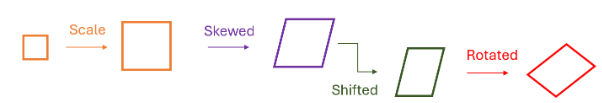
\includegraphics[width=0.7\linewidth,height=\textheight,keepaspectratio]{chapters/module_2/figures/geo_shapes.png}

}

\caption{\label{fig-geo}\emph{Graphical representation of scale, skew,
shift and rotate}}

\end{figure}%

\subsection{Similarity (Conformal)
Transformation}\label{similarity-conformal-transformation}

The Similarity Transformation, often referred to as the Helmert or
Conformal Transformation, is a specific form of the affine model that
applies translation, uniform scaling, and rotation, while preserving the
shape and angles of the original features Albrecht (2007). Unlike the
general affine transformation, which allows independent scaling and
shearing along the x and y axes, the similarity transformation
constrains the scale to be the same in both directions.

This model is particularly useful when: - The dataset requires alignment
but not distortion. - The original geometry must be preserved (for
example, engineering drawings, cadastral data, or orthophotos). - Only
uniform scale and rotation differences exist between the image and the
map coordinate system.

It is therefore ideal for survey mapping and local map registration
where shape fidelity is critical.

The general equations for a two-dimensional similarity transformation
are:

\[
X' = a + s(x\cos\theta - y\sin\theta)
\]

\[
Y' = b + s(x\sin\theta + y\cos\theta)
\]

where:

\begin{itemize}
\tightlist
\item
  (a, b) --- translation parameters (shift of origin)\\
\item
  (s) --- uniform scale factor\\
\item
  (\theta) --- rotation angle (in radians)
\end{itemize}

A minimum of two Ground Control Points (GCPs) is required to compute
these parameters, although more are typically used for redundancy and
error minimization via least-squares adjustment

\section{Affine Transformation}\label{affine-transformation}

Affine transformation is the simplest and most widely used
georeferencing model. It preserves straight lines and parallelism but
not necessarily distances or angles. This model is suitable for most
scanned maps, orthophotos, and satellite imagery where geometric
distortions are minimal and primarily linear. Affine transformation can
model translation, rotation, scaling, and shearing of the image. The
mathematical form of an affine transformation is linear and defined by
two equations:

\[
Y' = b_0 + b_1x + b_2y
\]

where:

\begin{itemize}
\tightlist
\item
  (a\_0, b\_0) = translation parameters (shifts in (x) and (y)
  directions)\\
\item
  (a\_1, b\_2) = scaling and rotation parameters\\
\item
  (a\_2, b\_1) = shearing parameters
\end{itemize}

A total of six parameters ((a\_0, a\_1, a\_2, b\_0, b\_1, b\_2)) are
required, which can be solved using \textbf{at least three Ground
Control Points (GCPs)}.

\subsection{Explanation of the
Components}\label{explanation-of-the-components}

\subsubsection{Translation}\label{translation}

Moves the image origin to a new location without changing its shape.

\[
X' = x + \Delta X
\]

\[
Y' = y + \Delta Y
\]

\subsubsection{Scaling}\label{scaling}

Changes the size of the image in the (x) or (y) direction.

\[
X' = s_x x
\]

\[
Y' = s_y y
\]

\subsubsection{Rotation}\label{rotation}

Rotates the image by an angle (\theta) around the origin.

\[
X' = x\cos\theta - y\sin\theta
\]

\[
Y' = x\sin\theta + y\cos\theta
\]

\subsubsection{Shearing}\label{shearing}

Distorts the image such that axes remain parallel but not perpendicular.

\[
X' = x + k_x y
\]

\[
Y' = y + k_y x
\]

where (k\_x) and (k\_y) are shear coefficients.

Combining all these transformations yields the \textbf{affine
transformation equations} shown above.

\part{Module 5: WebGIS}

\chapter{Introduction to WebGIS}\label{introduction-to-webgis}

\section{What is WebGIS?}\label{what-is-webgis}

WebGIS is a Geographic Information System that operates through the
internet. Unlike traditional desktop GIS, WebGIS enables users to
access, visualize, analyze, and share geospatial data directly from a
web browser without requiring specialized software. The primary goal of
WebGIS is the democratization of geospatial information by making it
widely accessible.

Key characteristics of WebGIS include the following:

\begin{itemize}
\tightlist
\item
  Accessible via the internet using standard web browsers\\
\item
  Requires minimal installation at the client side\\
\item
  Supports real-time data sharing and collaboration\\
\item
  Often built on open standards and free and open-source software (FOSS)
  (Mitchell, 2005)
\end{itemize}

\begin{figure}

\centering{

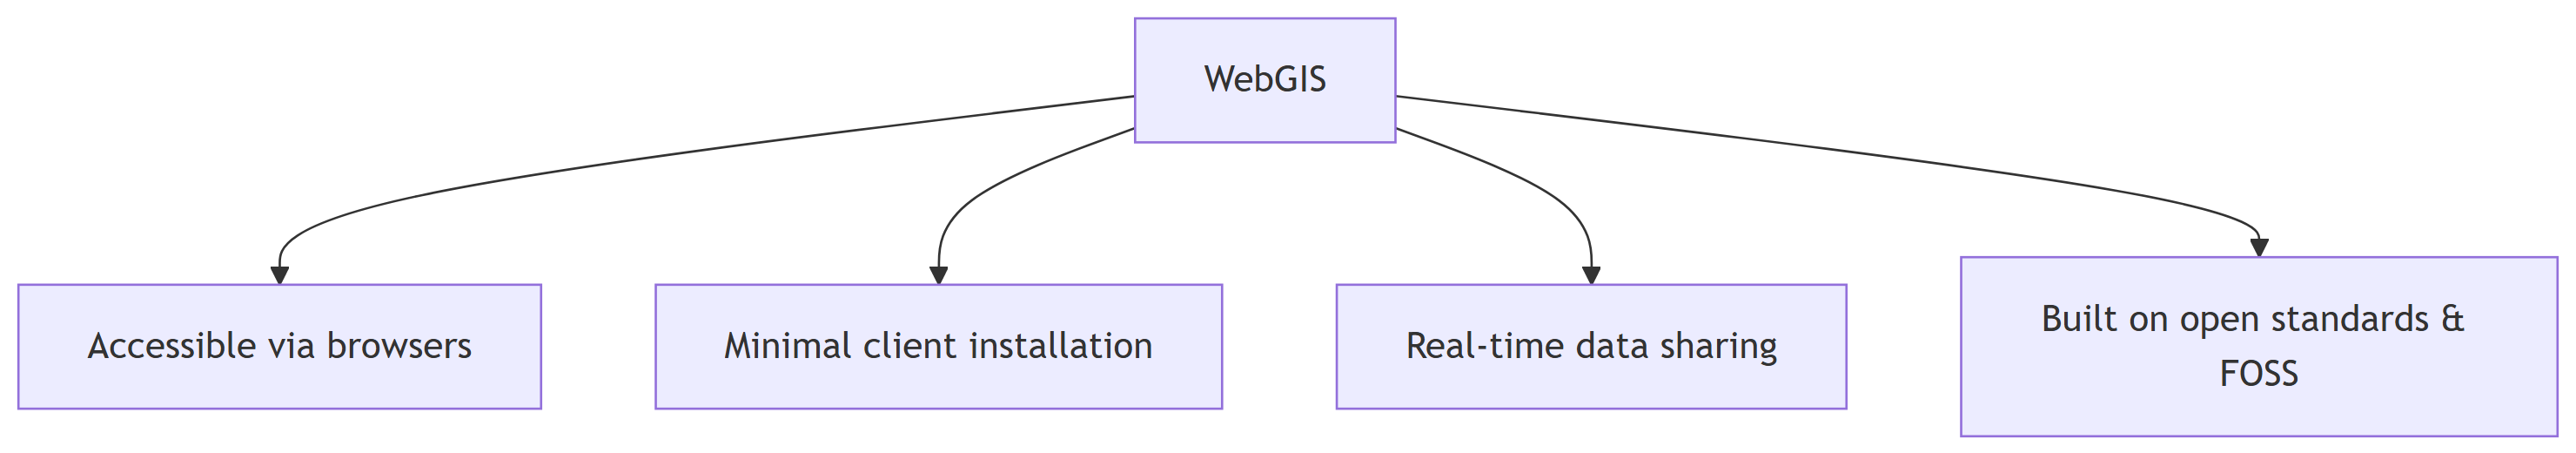
\includegraphics[width=11.7in,height=2.06in]{chapters/module_5/intro_webgis_files/figure-latex/mermaid-figure-1.png}

}

\caption{\label{fig-webgis-characteristics}Key characteristics of
WebGIS}

\end{figure}%

\section{Evolution of GIS to WebGIS}\label{evolution-of-gis-to-webgis}

The development of GIS began in the 1960s with desktop-based systems.
With the rise of the internet in the 1990s, GIS started moving online.
The availability of faster networks, open standards, and lightweight web
programming languages enabled the shift from standalone GIS to WebGIS.

Some important milestones in this evolution include:

\begin{itemize}
\tightlist
\item
  1960s--1980s: Desktop GIS focused on specialized users (Jones \&
  Purves, 2008)\\
\item
  1990s: Internet-enabled GIS applications emerged\\
\item
  2000s: Open Source GIS tools like MapServer and PostGIS supported
  online mapping (Mitchell, 2005)\\
\item
  2010s onwards: Cloud GIS and real-time WebGIS applications became
  mainstream
\end{itemize}

\section{WebGIS vs.~Traditional Desktop
GIS}\label{webgis-vs.-traditional-desktop-gis}

\begin{longtable}[]{@{}
  >{\raggedright\arraybackslash}p{(\linewidth - 4\tabcolsep) * \real{0.2785}}
  >{\raggedright\arraybackslash}p{(\linewidth - 4\tabcolsep) * \real{0.3291}}
  >{\raggedright\arraybackslash}p{(\linewidth - 4\tabcolsep) * \real{0.3924}}@{}}
\caption{\textbf{Comparison of Desktop GIS and WebGIS}}\tabularnewline
\toprule\noalign{}
\begin{minipage}[b]{\linewidth}\raggedright
Feature
\end{minipage} & \begin{minipage}[b]{\linewidth}\raggedright
Desktop GIS
\end{minipage} & \begin{minipage}[b]{\linewidth}\raggedright
WebGIS
\end{minipage} \\
\midrule\noalign{}
\endfirsthead
\toprule\noalign{}
\begin{minipage}[b]{\linewidth}\raggedright
Feature
\end{minipage} & \begin{minipage}[b]{\linewidth}\raggedright
Desktop GIS
\end{minipage} & \begin{minipage}[b]{\linewidth}\raggedright
WebGIS
\end{minipage} \\
\midrule\noalign{}
\endhead
\bottomrule\noalign{}
\endlastfoot
Accessibility & Installed on local machines & Accessible via web
browsers \\
User Base & Specialists and experts & General public and specialists \\
Data Sharing & Manual file exchange & Real-time data sharing online \\
Cost & Often commercial licenses & Many FOSS options available \\
\end{longtable}

\section{Components of a WebGIS}\label{components-of-a-webgis}

A WebGIS is composed of three main elements, each playing a critical
role in delivering geospatial services over the web:

\begin{itemize}
\tightlist
\item
  \textbf{Client-side (Frontend):} The user interface, often built with
  HTML, CSS, and JavaScript libraries such as Leaflet and OpenLayers\\
\item
  \textbf{Server-side (Backend):} Manages requests, processes data, and
  delivers maps using tools like GeoServer and MapServer\\
\item
  \textbf{Database:} Stores and manages spatial data, with common FOSS
  options including PostGIS and Spatialite (Mitchell, 2005)
\end{itemize}

\begin{figure}

\centering{


\includegraphics[width=2.88in,height=3.4in]{chapters/module_5/intro_webgis_files/figure-latex/mermaid-figure-2.png}

}

\caption{\label{fig-components-webgis}Basic components of a WebGIS
system}

\end{figure}%

\section{Importance of WebGIS}\label{importance-of-webgis}

The importance of WebGIS lies in its ability to extend geospatial
capabilities beyond specialists. It plays a crucial role in governance,
research, and community participation.

Key benefits of WebGIS include:

\begin{itemize}
\tightlist
\item
  Enhances accessibility of geospatial data (Jones \& Purves, 2008)\\
\item
  Facilitates collaboration across disciplines and locations\\
\item
  Supports decision-making in urban planning, disaster management, and
  environmental monitoring\\
\item
  Promotes open data initiatives and citizen science
\end{itemize}

\section{Examples of WebGIS
Applications}\label{examples-of-webgis-applications}

Many well-known platforms demonstrate the capabilities of WebGIS. Some
examples are:

\begin{itemize}
\tightlist
\item
  \textbf{\href{https://maps.google.com}{Google Maps}:} A popular
  navigation and mapping platform for general use\\
\item
  \textbf{\href{https://www.openstreetmap.org}{OpenStreetMap}:} A
  collaborative, open-source mapping initiative\\
\item
  \textbf{Geoportals (e.g., \href{https://earthexplorer.usgs.gov/}{USGS
  EarthExplorer}, \href{https://scihub.copernicus.eu/}{European
  Copernicus Open Access Hub}):}\\
\item
  \textbf{\href{https://www.hotosm.org/}{Humanitarian OpenStreetMap Team
  (HOT)}:} Community-driven mapping for disaster response.\\
\item
  \textbf{\href{https://geonode.worldbank.org/}{World Bank GeoNode}:}
  Open platform for global development and spatial data sharing.
  Platforms from governments and universities offering public geospatial
  data (Jones \& Purves, 2008)
\end{itemize}

\section{Conclusion}\label{conclusion-6}

This introductory chapter has outlined the meaning, evolution, and
importance of WebGIS. It explained how WebGIS differs from traditional
GIS and described the components that make it operational. The
importance of WebGIS lies in enhancing accessibility, supporting
collaborative research, and encouraging participatory mapping through
FOSS and open data initiatives.

As the internet continues to influence data accessibility, WebGIS is
becoming central to modern geospatial practices. The next chapter will
introduce the \textbf{fundamental web principles} that underpin WebGIS.
Understanding how the web functions, including client-server
communication and the role of protocols, provides the foundation for
grasping how geospatial data is shared and visualized online.

\chapter{Web Principles for GIS}\label{web-principles-for-gis}

\section{Introduction}\label{introduction-2}

To understand WebGIS, it is essential to first explore the fundamental
principles of how the web functions. WebGIS applications rely on
internet protocols, client-server communication, and structured
architectures that enable efficient sharing and visualization of spatial
data. This chapter introduces these underlying web principles and
explains their role in enabling WebGIS.

\section{The Internet and the World Wide
Web}\label{the-internet-and-the-world-wide-web}

The internet is a global network of interconnected computers, while the
World Wide Web (WWW) is a system of interlinked documents accessed via
the internet. The web acts as the primary platform for delivering GIS
data and applications.

Important distinctions include:

\begin{itemize}
\tightlist
\item
  \textbf{Internet:} Infrastructure that connects networks worldwide.\\
\item
  \textbf{World Wide Web:} Collection of linked resources accessible
  through HTTP.
\end{itemize}

The emergence of the WWW in the early 1990s revolutionized GIS by
enabling online access to spatial data and maps (Jones \& Purves, 2008).

\section{Client-Server Architecture}\label{client-server-architecture}

Web applications, including WebGIS, are based on client-server
architecture. In this model:\\
- \textbf{Client:} The user's browser or application that requests
resources (e.g., Google Chrome, Mozilla Firefox, QGIS with web
plugins).\\
- \textbf{Server:} A machine that stores, processes, and serves
requested data (e.g., Apache HTTP Server, GeoServer, MapServer).

\begin{figure}

\centering{


\includegraphics[width=7.63in,height=3.61in]{chapters/module_5/webgis_principles_files/figure-latex/mermaid-figure-1.png}

}

\caption{\label{fig-client-server}Client-server interaction in WebGIS}

\end{figure}%

\subsection{Types of Clients}\label{types-of-clients}

\begin{itemize}
\tightlist
\item
  \textbf{Thin Clients:} Depend on the server for most processing tasks
  (e.g., browsers running Leaflet, OpenLayers).\\
\item
  \textbf{Thick Clients:} Perform processing locally while interacting
  with the server (e.g., QGIS with WMS/WFS, ArcGIS Pro).
\end{itemize}

\begin{figure}

\centering{

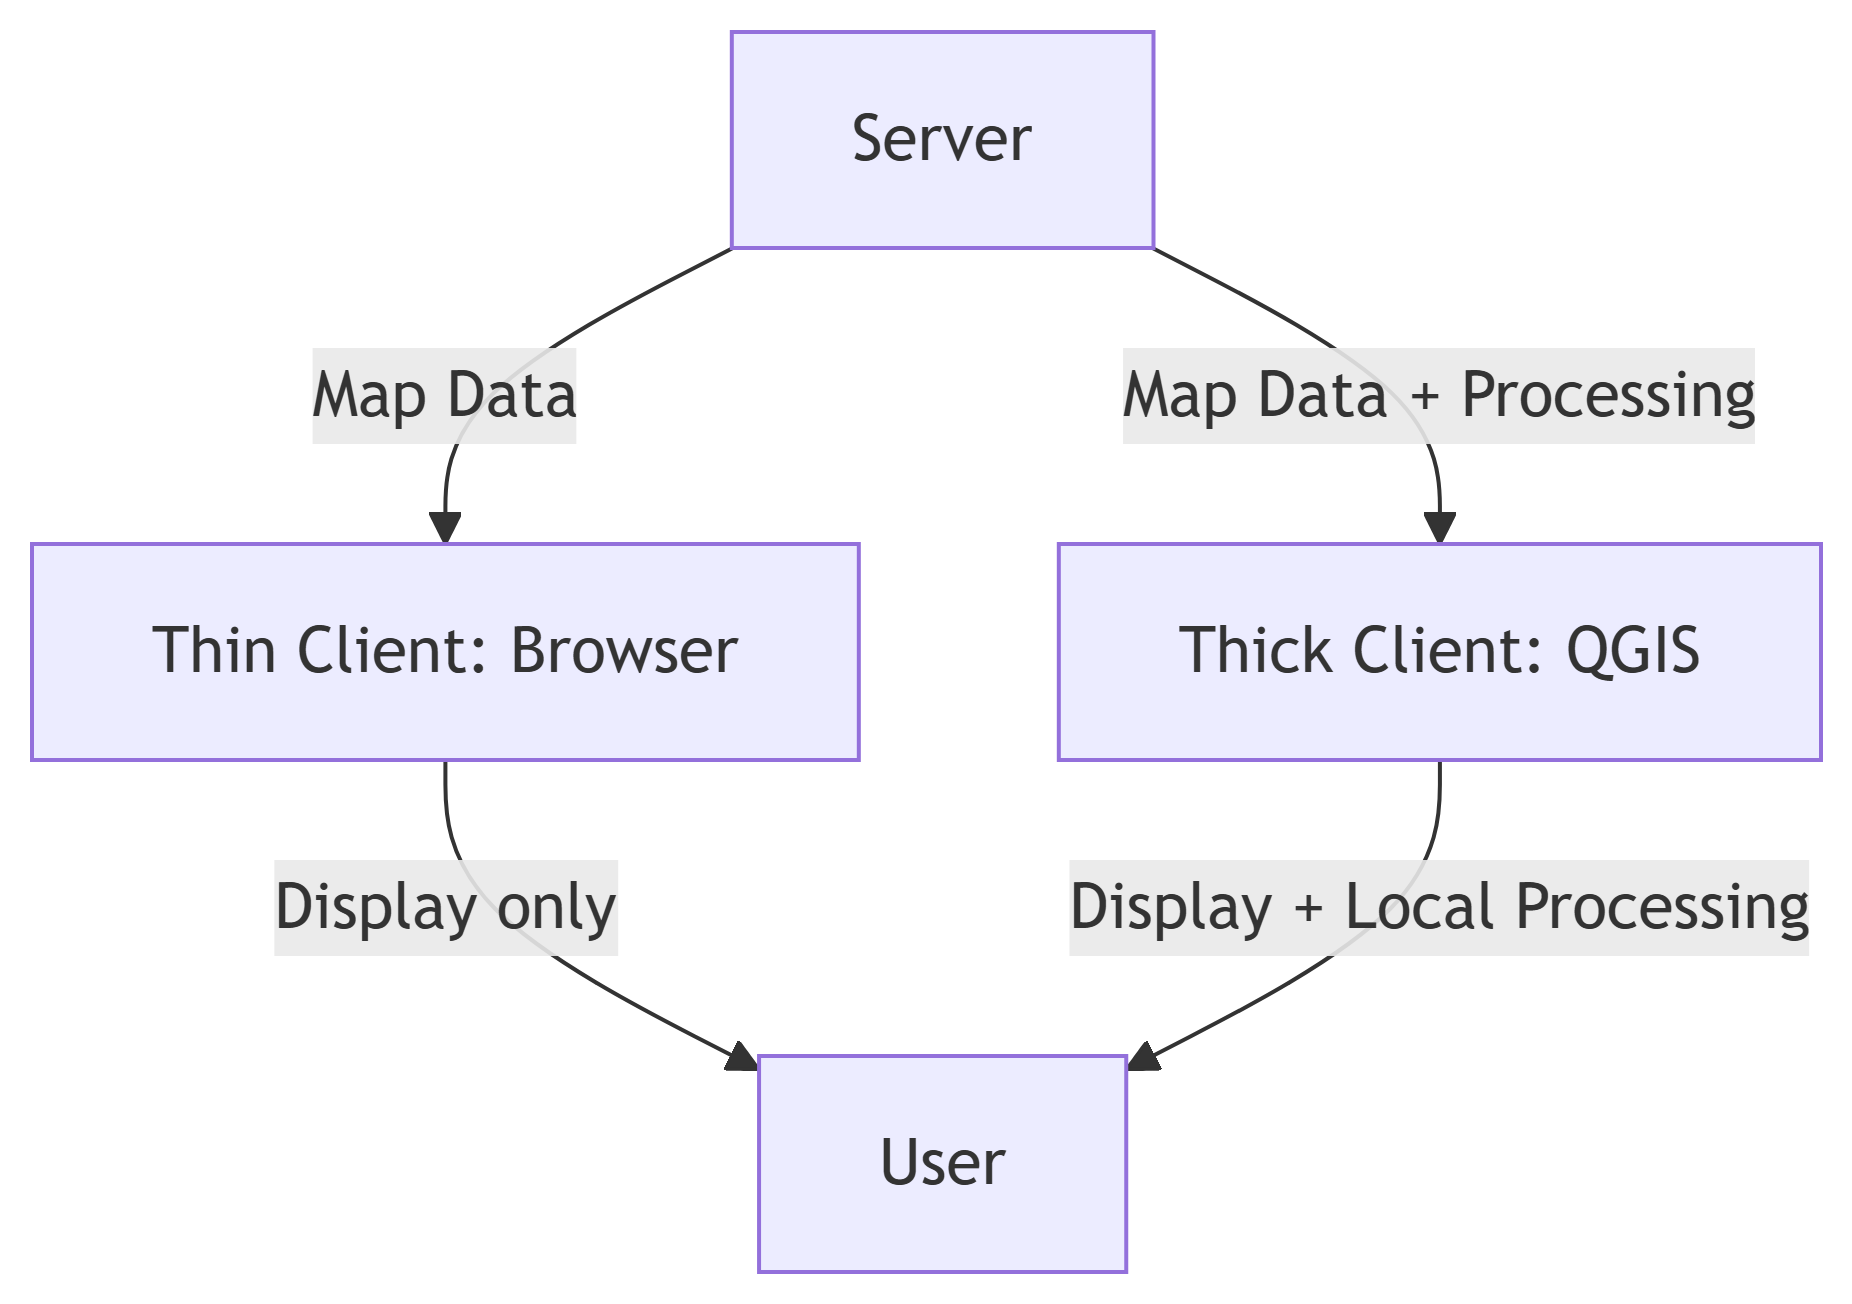
\includegraphics[width=4.83in,height=3.4in]{chapters/module_5/webgis_principles_files/figure-latex/mermaid-figure-4.png}

}

\caption{\label{fig-thin-thick}Thin versus thick clients in WebGIS}

\end{figure}%

\section{HTTP Protocol}\label{http-protocol}

The Hypertext Transfer Protocol (HTTP) is the standard for communication
between clients and servers.

Common methods include:

\begin{itemize}
\tightlist
\item
  \textbf{GET:} Request information (e.g., fetch a map layer).\\
\item
  \textbf{POST:} Submit data to the server (e.g., upload spatial
  data).\\
\item
  \textbf{PUT:} Update or replace an existing resource.\\
\item
  \textbf{DELETE:} Remove a resource from the server.
\end{itemize}

\begin{figure}

\centering{


\includegraphics[width=5.96in,height=2.7in]{chapters/module_5/webgis_principles_files/figure-latex/mermaid-figure-3.png}

}

\caption{\label{fig-http-flow}HTTP request and response flow in WebGIS}

\end{figure}%

\section{Three-Tier Web Architecture}\label{three-tier-web-architecture}

Most WebGIS applications adopt a three-tier architecture:

\begin{enumerate}
\def\labelenumi{\arabic{enumi}.}
\tightlist
\item
  \textbf{Presentation Layer:} User interface (browser, mobile app).\\
\item
  \textbf{Logic Layer:} Server-side scripts (e.g., Python Flask, PHP,
  Node.js).\\
\item
  \textbf{Data Layer:} Database storing spatial data (e.g., PostGIS,
  MongoDB with geospatial extensions).
\end{enumerate}

\begin{figure}

\centering{


\includegraphics[width=2.88in,height=3.4in]{chapters/module_5/webgis_principles_files/figure-latex/mermaid-figure-2.png}

}

\caption{\label{fig-three-tier}Three-tier architecture of WebGIS}

\end{figure}%

\section{Conclusion}\label{conclusion-7}

This chapter explained the basic web principles that form the foundation
of WebGIS. By understanding the internet, client-server communication,
HTTP protocols, and three-tier architecture, it becomes clear how WebGIS
applications function effectively. The distinction between thin and
thick clients further illustrates how processing responsibilities are
distributed in different setups. Data formats such as XML, JSON, and GML
ensure interoperability across platforms.

In the next chapter, we will explore \textbf{Geospatial Web Services},
which build upon these principles to provide spatial data and
functionality over the internet.

\chapter{Geospatial Web Services}\label{geospatial-web-services}

\section{Introduction}\label{introduction-3}

Geospatial Web Services are the backbone of WebGIS. They provide a
standardized way for servers to share spatial data and functionalities
with clients across the internet. These services follow open standards,
mainly from the Open Geospatial Consortium (OGC), ensuring
interoperability between different software systems. This chapter
introduces the concepts of web services, their types, and their
applications in WebGIS.

\section{From Websites to Web
Services}\label{from-websites-to-web-services}

Traditional websites deliver content for human interaction, whereas web
services are designed for communication between machines. Geospatial web
services expose functionalities such as map visualization, feature
querying, or spatial analysis through standard protocols (Jones \&
Purves, 2008).

\subsection{Characteristics of Web
Services}\label{characteristics-of-web-services}

\begin{itemize}
\tightlist
\item
  Machine-to-machine interaction\\
\item
  Platform independent\\
\item
  Accessible using standard protocols (HTTP, HTTPS)\\
\item
  Responses formatted in XML, JSON, or other open standards
\end{itemize}

\begin{figure}

\centering{


\includegraphics[width=7.58in,height=3.61in]{chapters/module_5/webgis_services_files/figure-latex/mermaid-figure-1.png}

}

\caption{\label{fig-webservice-flow}General flow of a geospatial web
service request}

\end{figure}%

\section{Types of Geospatial Web
Services}\label{types-of-geospatial-web-services}

The Open Geospatial Consortium (OGC) defines several service standards.
Traditionally, WebGIS relied on services such as WMS,WFS, WCS and WPS.
However, these are now considered \textbf{legacy standards}, with the
\textbf{OGC API family} being the modern alternative.

\subsection{Legacy standards}\label{legacy-standards}

\begin{itemize}
\tightlist
\item
  \textbf{Web Map Service (WMS):} Provides map images rendered from
  geospatial data.\\
\item
  \textbf{Web Feature Service (WFS):} Shares vector features with
  attributes in formats like GML or GeoJSON.\\
\item
  \textbf{Web Coverage Service (WCS):} Provides raster data (e.g.,
  satellite imagery, elevation models).\\
\item
  \textbf{Catalog Service for the Web (CSW):} Supports search and
  discovery of geospatial metadata.\\
\item
  \textbf{Web Processing Service (WPS):} Exposes geospatial processing
  operations as web services, allowing distributed computation.
\end{itemize}

\begin{figure}

\centering{

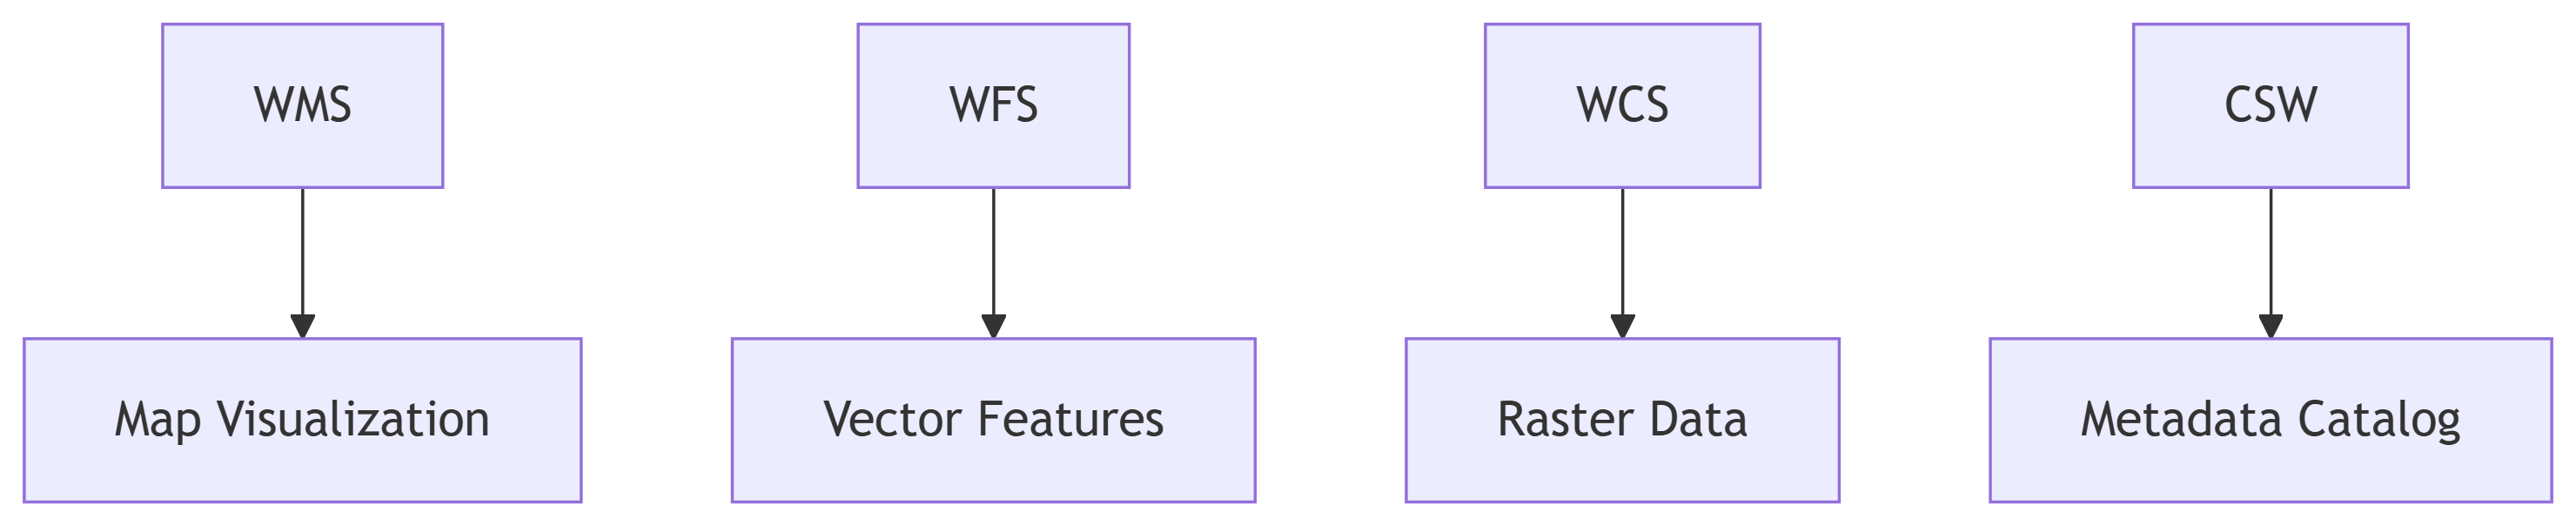
\includegraphics[width=8.88in,height=1.81in]{chapters/module_5/webgis_services_files/figure-latex/mermaid-figure-2.png}

}

\caption{\label{fig-ogc-services}Core OGC geospatial web service types}

\end{figure}%

\subsection{Modern alternative}\label{modern-alternative}

\begin{itemize}
\tightlist
\item
  \textbf{OGC API - Features:} Successor to WFS, uses REST and
  JSON/GeoJSON for lightweight feature access.\\
\item
  \textbf{OGC API - Maps:} Successor to WMS, uses REST and JSON/GeoJSON
  for lightweight feature access.\\
\item
  \textbf{OGC API - Tiles :} Provides tiles of vector and raster data,
  successor to WMTS.\\
\item
  \textbf{OGC API - Processes :} Successor to WPS, enables remote
  execution of geoprocessing tasks through REST APIs.
\end{itemize}

\section{Data Formats in Web
Services}\label{data-formats-in-web-services}

Web services rely on structured data formats for communication:

\begin{itemize}
\tightlist
\item
  \textbf{XML/GML:} Used in WFS and CSW for structured geospatial
  information.\\
\item
  \textbf{JSON/GeoJSON:} Lightweight and widely used for web-based
  vector data.\\
\item
  \textbf{PNG/JPEG:} Common image formats for WMS map rendering.
\end{itemize}

These formats allow integration between diverse systems and client
applications (Mitchell, 2005).

\section{Example Software for Web
Services}\label{example-software-for-web-services}

\begin{itemize}
\tightlist
\item
  \textbf{Server-side:} GeoServer, MapServer, deegree\\
\item
  \textbf{Client-side:} OpenLayers, Leaflet, Cesium
\end{itemize}

GeoServer and MapServer can publish data as WMS, WFS, and WCS, while
OpenLayers and Leaflet can consume and visualize this data in web
browsers.

\subsection{Practical Example: Accessing OGC
Services}\label{practical-example-accessing-ogc-services}

Below is an example showing how to use \textbf{Leaflet} to access both a
legacy WMS and a modern OGC API - Features service.

\subsubsection{Legacy WMS Example}\label{legacy-wms-example}

\begin{Shaded}
\begin{Highlighting}[]
\KeywordTok{var}\NormalTok{ map }\OperatorTok{=}\NormalTok{ L}\OperatorTok{.}\FunctionTok{map}\NormalTok{(}\StringTok{\textquotesingle{}map\textquotesingle{}}\NormalTok{)}\OperatorTok{.}\FunctionTok{setView}\NormalTok{([}\FloatTok{25.0}\OperatorTok{,} \FloatTok{84.0}\NormalTok{]}\OperatorTok{,} \DecValTok{6}\NormalTok{)}\OperatorTok{;}

\CommentTok{// Public ISRO Bhuvan WMS (Land Use Land Cover thematic layer)}
\NormalTok{L}\OperatorTok{.}\AttributeTok{tileLayer}\OperatorTok{.}\FunctionTok{wms}\NormalTok{(}\StringTok{"https://bhuvan{-}vec2.nrsc.gov.in/bhuvan/wms"}\OperatorTok{,}\NormalTok{ \{}
  \DataTypeTok{layers}\OperatorTok{:} \StringTok{\textquotesingle{}lulc:BR\_LULC50K\_1112\textquotesingle{}}\OperatorTok{,}
  \DataTypeTok{format}\OperatorTok{:} \StringTok{\textquotesingle{}image/png\textquotesingle{}}\OperatorTok{,}
  \DataTypeTok{transparent}\OperatorTok{:} \KeywordTok{true}\OperatorTok{,}
  \DataTypeTok{attribution}\OperatorTok{:} \StringTok{"Map data © ISRO Bhuvan"}
\NormalTok{\})}\OperatorTok{.}\FunctionTok{addTo}\NormalTok{(map)}\OperatorTok{;}
\end{Highlighting}
\end{Shaded}

\subsubsection{Modern OGC API - Features
Example}\label{modern-ogc-api---features-example}

\begin{Shaded}
\begin{Highlighting}[]
\FunctionTok{fetch}\NormalTok{(}\StringTok{"https://demo.pygeoapi.io/master/collections/lakes/items"}\NormalTok{)}
  \OperatorTok{.}\FunctionTok{then}\NormalTok{(response }\KeywordTok{=\textgreater{}}\NormalTok{ response}\OperatorTok{.}\FunctionTok{json}\NormalTok{())}
  \OperatorTok{.}\FunctionTok{then}\NormalTok{(data }\KeywordTok{=\textgreater{}}\NormalTok{ \{}
\NormalTok{      L}\OperatorTok{.}\FunctionTok{geoJSON}\NormalTok{(data}\OperatorTok{,}\NormalTok{ \{}
          \DataTypeTok{onEachFeature}\OperatorTok{:} \KeywordTok{function}\NormalTok{ (feature}\OperatorTok{,}\NormalTok{ layer) \{}
\NormalTok{              layer}\OperatorTok{.}\FunctionTok{bindPopup}\NormalTok{(}\StringTok{"Lake: "} \OperatorTok{+}\NormalTok{ feature}\OperatorTok{.}\AttributeTok{properties}\OperatorTok{.}\AttributeTok{name}\NormalTok{)}\OperatorTok{;}
\NormalTok{          \}}
\NormalTok{      \})}\OperatorTok{.}\FunctionTok{addTo}\NormalTok{(map)}\OperatorTok{;}
\NormalTok{  \})}\OperatorTok{;}
\end{Highlighting}
\end{Shaded}

In this example, the OGC API - Features endpoint delivers
\textbf{GeoJSON directly}, which is easily integrated into Leaflet
without complex parsing, making it more lightweight compared to WMS/WFS.

\section{Conclusion}\label{conclusion-8}

Geospatial Web Services provide the essential link between clients and
geospatial databases, enabling data visualization, feature access, and
analysis over the internet. By adopting OGC standards such as WMS, WFS,
WCS, and CSW, WebGIS ensures interoperability across diverse systems.
The next chapter will focus on \textbf{Open Source Web Mapping Tools},
where these services are implemented and visualized using free and
open-source software.

\chapter{WebGIS Tools and Application
Design}\label{webgis-tools-and-application-design}

\section{Introduction}\label{introduction-4}

Developing a WebGIS system requires robust tools, thoughtful design
practices, and the ability to integrate heterogeneous data sources. This
chapter presents the open-source ecosystem, methods for designing
scalable applications, and mashup strategies that combine multiple
services into integrated geospatial platforms. It emphasizes the role of
Free and Open Source Software (FOSS) as the foundation for accessible
and collaborative WebGIS.

\begin{center}\rule{0.5\linewidth}{0.5pt}\end{center}

\section{The Role of FOSS in WebGIS}\label{the-role-of-foss-in-webgis}

\subsection{Web APIs in the FOSS
Ecosystem}\label{web-apis-in-the-foss-ecosystem}

An important contribution of FOSS to WebGIS is the development of
\textbf{Web APIs} that expose geospatial functionality over the
internet.\\
- \textbf{Leaflet API:} Offers simple functions to add layers, markers,
and controls in a few lines of code.\\
- \textbf{OpenLayers API:} Provides more advanced methods to handle OGC
standards and tiled data.\\
- \textbf{GeoServer REST API:} Allows publishing, styling, and managing
geospatial layers programmatically.\\
- \textbf{OGC API standards:} Designed as modern RESTful APIs using JSON
and GeoJSON, making them lightweight alternatives to legacy WMS and WFS.

These APIs allow developers to build applications that are modular,
interoperable, and cloud-ready.

\begin{figure}

\centering{

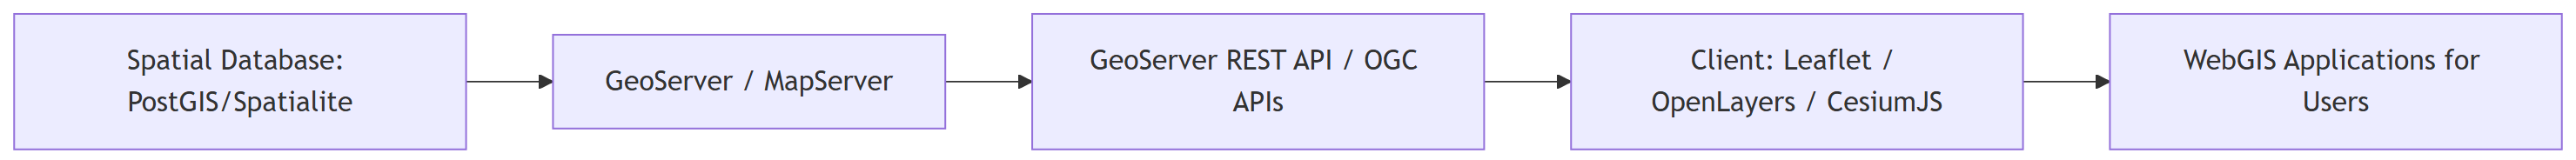
\includegraphics[width=15.43in,height=0.98in]{chapters/module_5/webgis_tools_and_app_files/figure-latex/mermaid-figure-1.png}

}

\caption{\label{fig-webapi-ecosystem}Role of Web APIs in connecting
databases, servers, and client applications}

\end{figure}%

FOSS solutions dominate WebGIS development due to their
cost-effectiveness, flexibility, and support for open standards. Unlike
proprietary platforms, FOSS encourages community-driven innovation and
interoperability through the Open Geospatial Consortium (OGC) standards
such as WMS, WFS, and WCS.

\subsection{Why FOSS?}\label{why-foss}

\begin{itemize}
\tightlist
\item
  \textbf{Cost efficiency:} Free licensing removes financial barriers.\\
\item
  \textbf{Transparency:} Open code allows customization and auditing.\\
\item
  \textbf{Community support:} Large global communities maintain and
  extend functionality.\\
\item
  \textbf{Interoperability:} Adherence to OGC standards ensures
  cross-platform compatibility.
\end{itemize}

\begin{figure}

\centering{

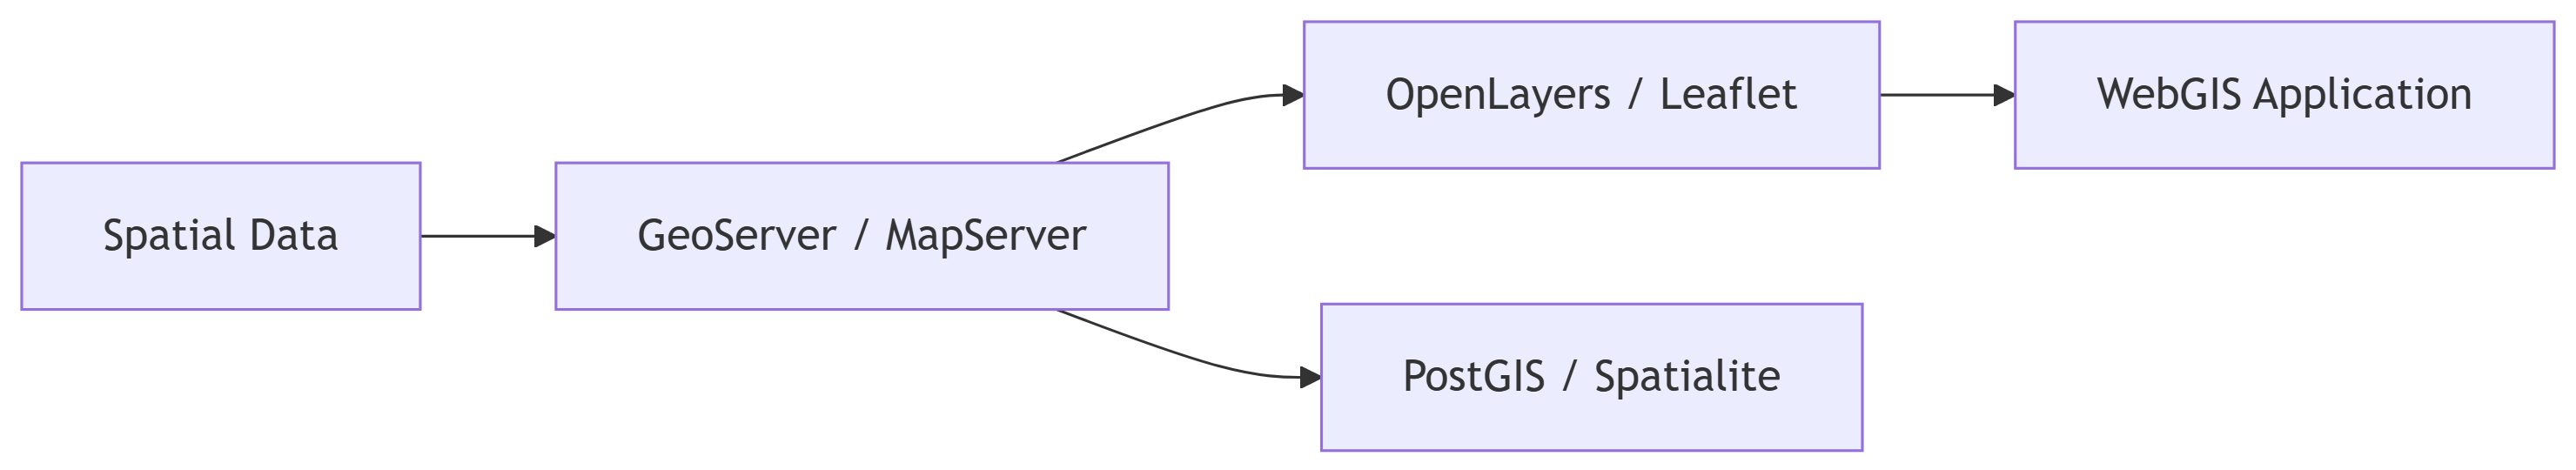
\includegraphics[width=9.89in,height=1.81in]{chapters/module_5/webgis_tools_and_app_files/figure-latex/mermaid-figure-7.png}

}

\caption{\label{fig-foss-ecosystem}The FOSS ecosystem in WebGIS}

\end{figure}%

\begin{center}\rule{0.5\linewidth}{0.5pt}\end{center}

\section{Map Servers}\label{map-servers}

Map servers handle the publication and delivery of geospatial data as
standardized services.

\begin{itemize}
\tightlist
\item
  \textbf{GeoServer:} Known for ease of use, strong OGC compliance, and
  support for PostGIS.\\
\item
  \textbf{MapServer:} High-performance rendering engine with flexibility
  for advanced cartography.\\
\item
  \textbf{deegree:} Enterprise-level server with strong metadata
  management.
\end{itemize}

\begin{center}\rule{0.5\linewidth}{0.5pt}\end{center}

\section{Client Libraries}\label{client-libraries}

Client-side libraries handle visualization and interactivity.

\begin{itemize}
\tightlist
\item
  \textbf{OpenLayers:} Comprehensive support for OGC standards, powerful
  for enterprise-grade projects.\\
\item
  \textbf{Leaflet:} Lightweight and beginner-friendly, widely used for
  rapid application development.\\
\item
  \textbf{CesiumJS:} Specialized for 3D mapping and virtual globes.
\end{itemize}

\begin{figure}

\centering{

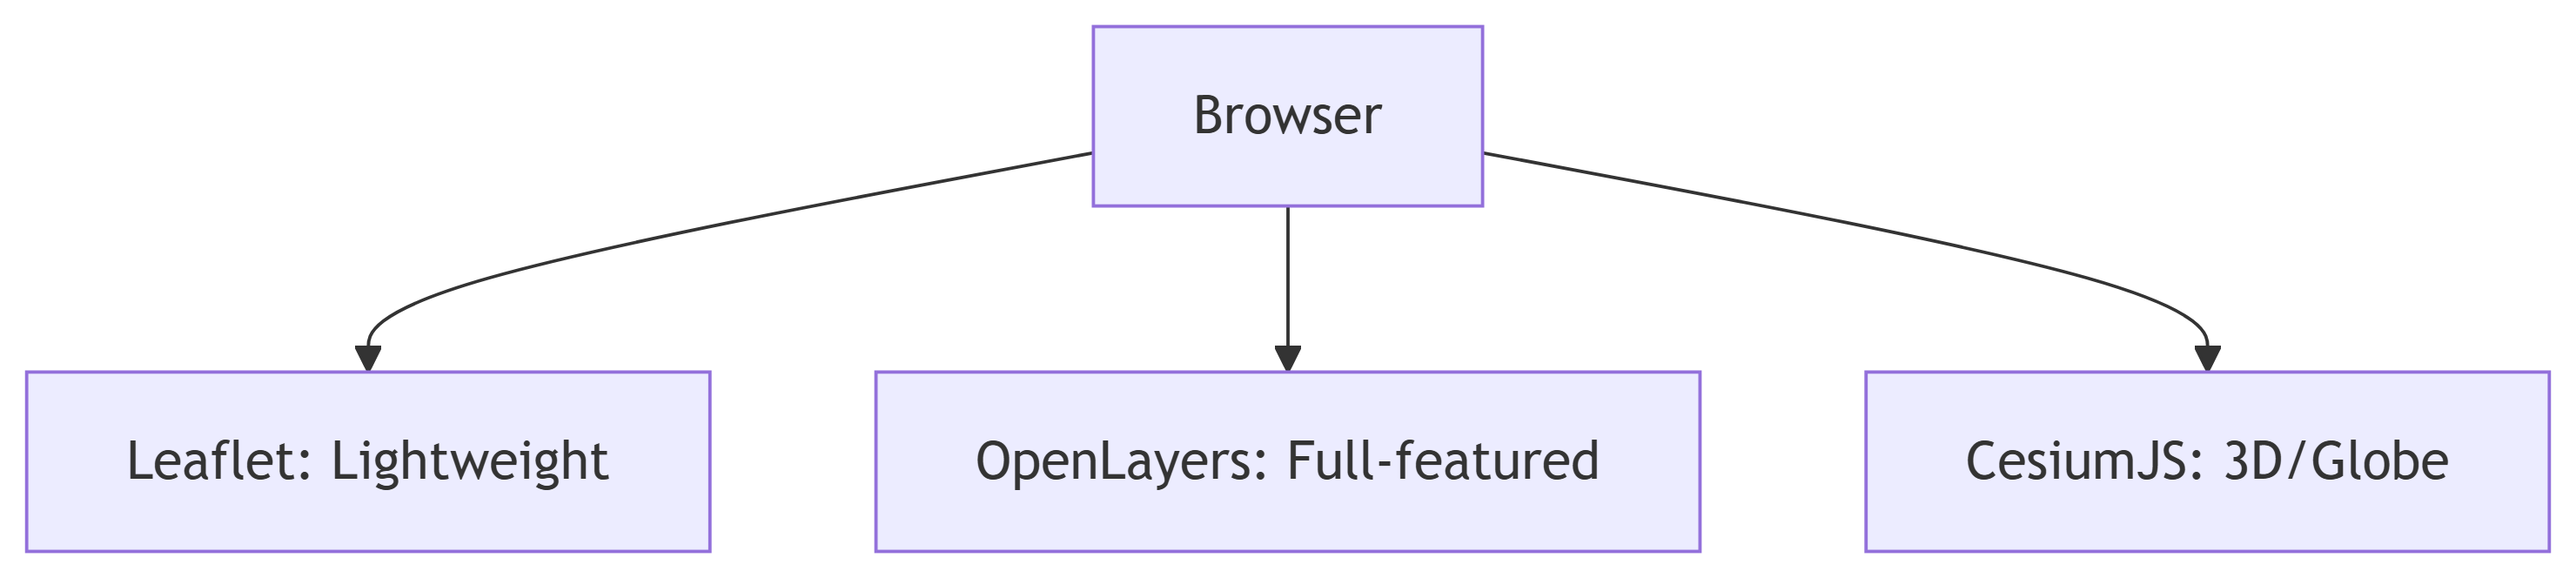
\includegraphics[width=8.08in,height=1.81in]{chapters/module_5/webgis_tools_and_app_files/figure-latex/mermaid-figure-6.png}

}

\caption{\label{fig-client-libraries}Client-side libraries for
visualization in WebGIS}

\end{figure}%

\begin{center}\rule{0.5\linewidth}{0.5pt}\end{center}

\section{Databases for WebGIS}\label{databases-for-webgis}

Spatial databases store and query geospatial data efficiently.

\begin{itemize}
\tightlist
\item
  \textbf{PostGIS:} An extension of PostgreSQL offering spatial indexing
  (GiST, R-Tree) and functions (ST\_Buffer, ST\_Intersection).\\
\item
  \textbf{Spatialite:} SQLite-based lightweight alternative for portable
  projects.
\end{itemize}

\subsection{Example PostGIS Query}\label{example-postgis-query}

\begin{Shaded}
\begin{Highlighting}[]
\KeywordTok{SELECT}\NormalTok{ name, ST\_Area(geom) }
\KeywordTok{FROM}\NormalTok{ landuse }
\KeywordTok{WHERE} \KeywordTok{type} \OperatorTok{=} \StringTok{\textquotesingle{}forest\textquotesingle{}}\NormalTok{;}
\end{Highlighting}
\end{Shaded}

\begin{center}\rule{0.5\linewidth}{0.5pt}\end{center}

\section{Designing WebGIS
Applications}\label{designing-webgis-applications}

A WebGIS architecture involves three main layers: client, server, and
database. Scalability, security, and usability are critical design
principles.

\begin{figure}

\centering{


\includegraphics[width=2.88in,height=4.23in]{chapters/module_5/webgis_tools_and_app_files/figure-latex/mermaid-figure-5.png}

}

\caption{\label{fig-webgis-architecture}Architecture of a WebGIS
application}

\end{figure}%

\subsection{Key Considerations}\label{key-considerations}

\begin{itemize}
\tightlist
\item
  \textbf{System requirements:} Ensure bandwidth and server capacity.\\
\item
  \textbf{Security:} HTTPS, authentication, and role-based access
  control.\\
\item
  \textbf{Scalability:} Caching with GeoWebCache, load balancing in
  cloud environments.
\end{itemize}

\subsection{Layers in WebGIS}\label{layers-in-webgis}

\begin{itemize}
\tightlist
\item
  \textbf{Basemap Layers:} Provide context (e.g., OpenStreetMap).\\
\item
  \textbf{Operational Layers:} Application-specific overlays (e.g.,
  disaster hotspots, utilities).
\end{itemize}

\begin{figure}

\centering{

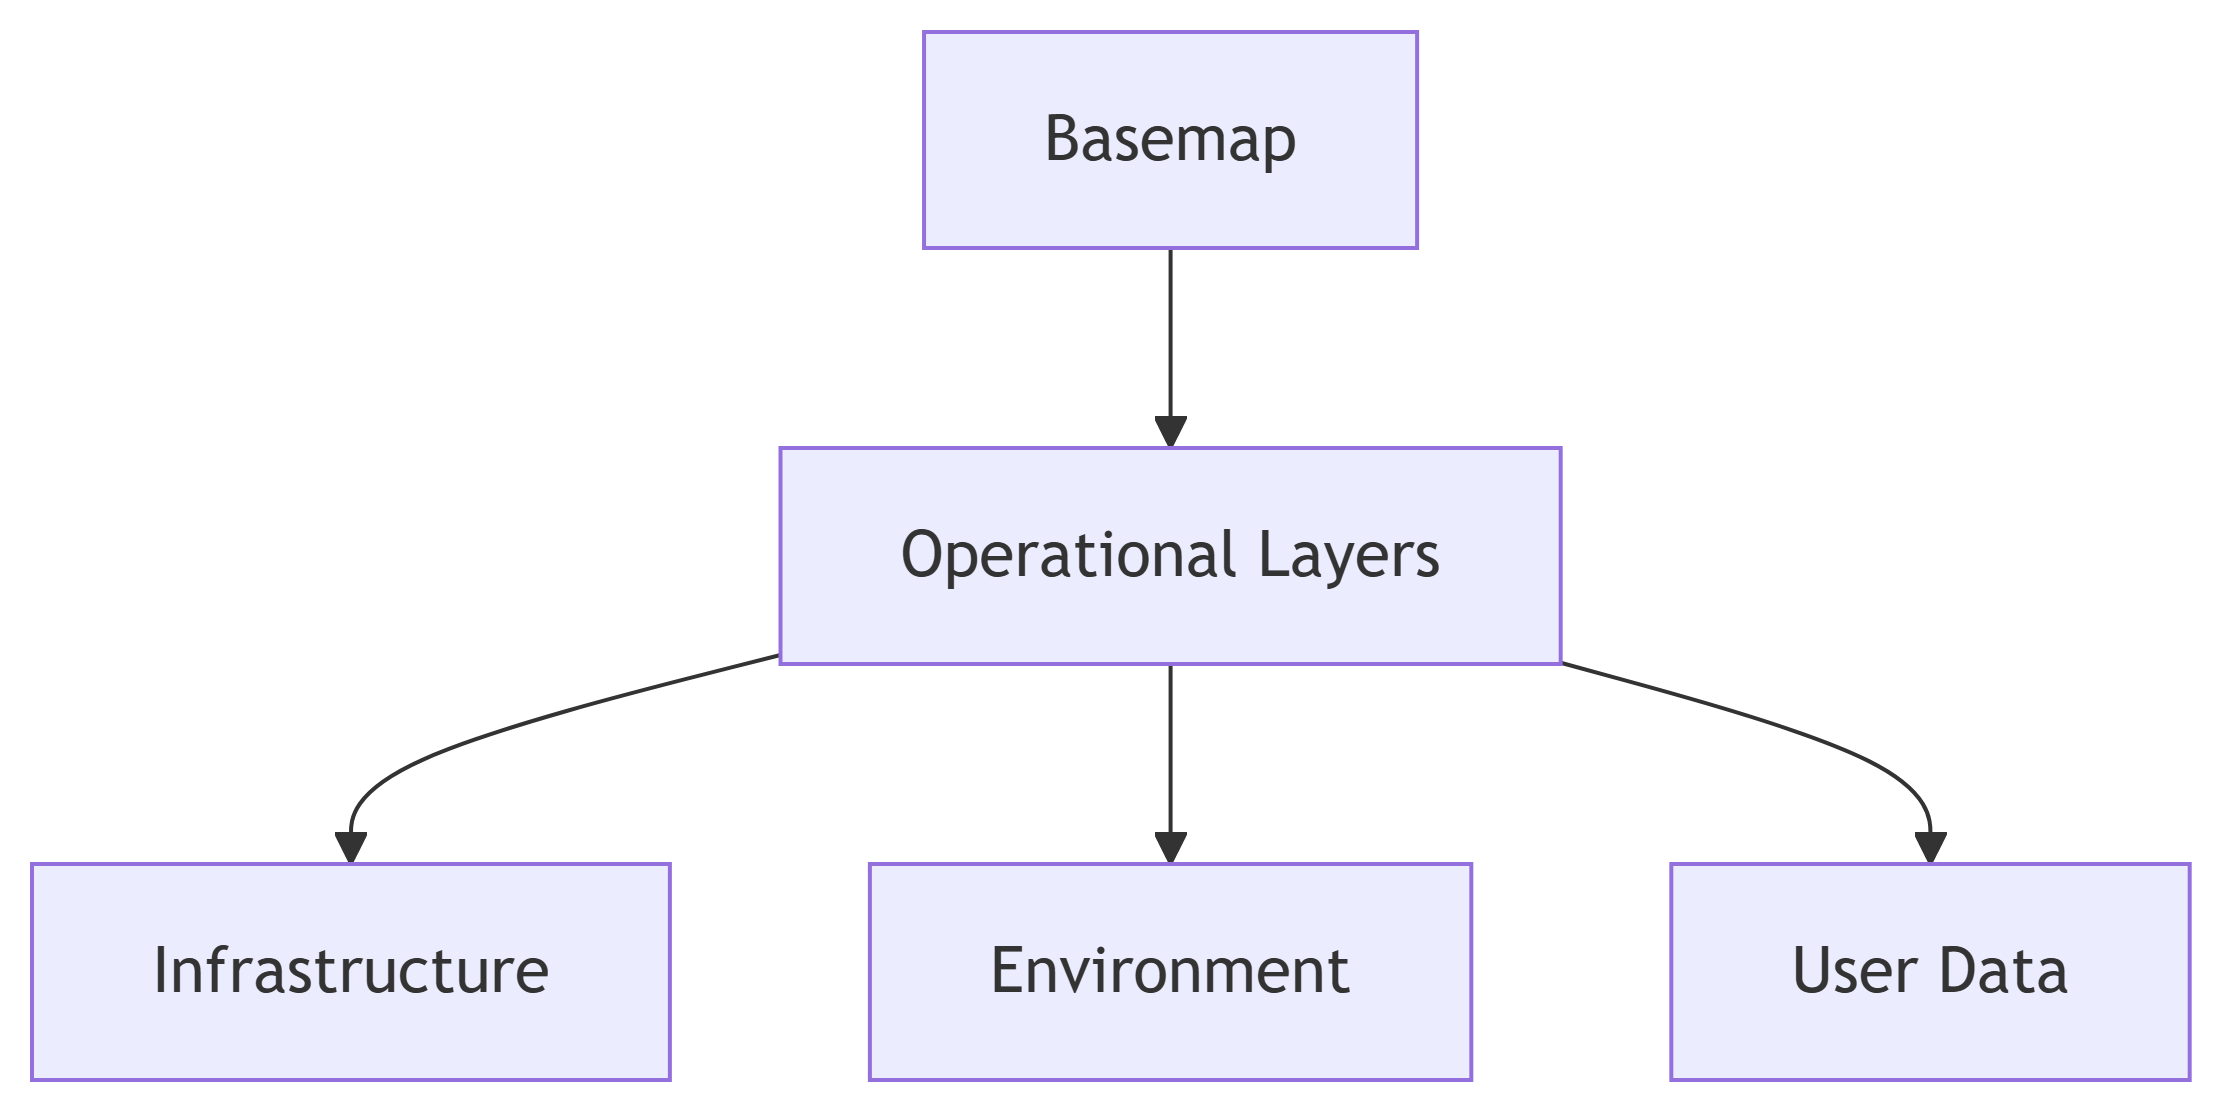
\includegraphics[width=5.79in,height=2.9in]{chapters/module_5/webgis_tools_and_app_files/figure-latex/mermaid-figure-4.png}

}

\caption{\label{fig-layer-structure}Basemap and operational layers in
WebGIS}

\end{figure}%

\begin{center}\rule{0.5\linewidth}{0.5pt}\end{center}

\section{Mashups in WebGIS}\label{mashups-in-webgis}

Mashups combine data from multiple APIs and services, enriching WebGIS
functionality. They became popular with the introduction of the Google
Maps API (2005) and now integrate real-time and open data.

\begin{figure}

\centering{

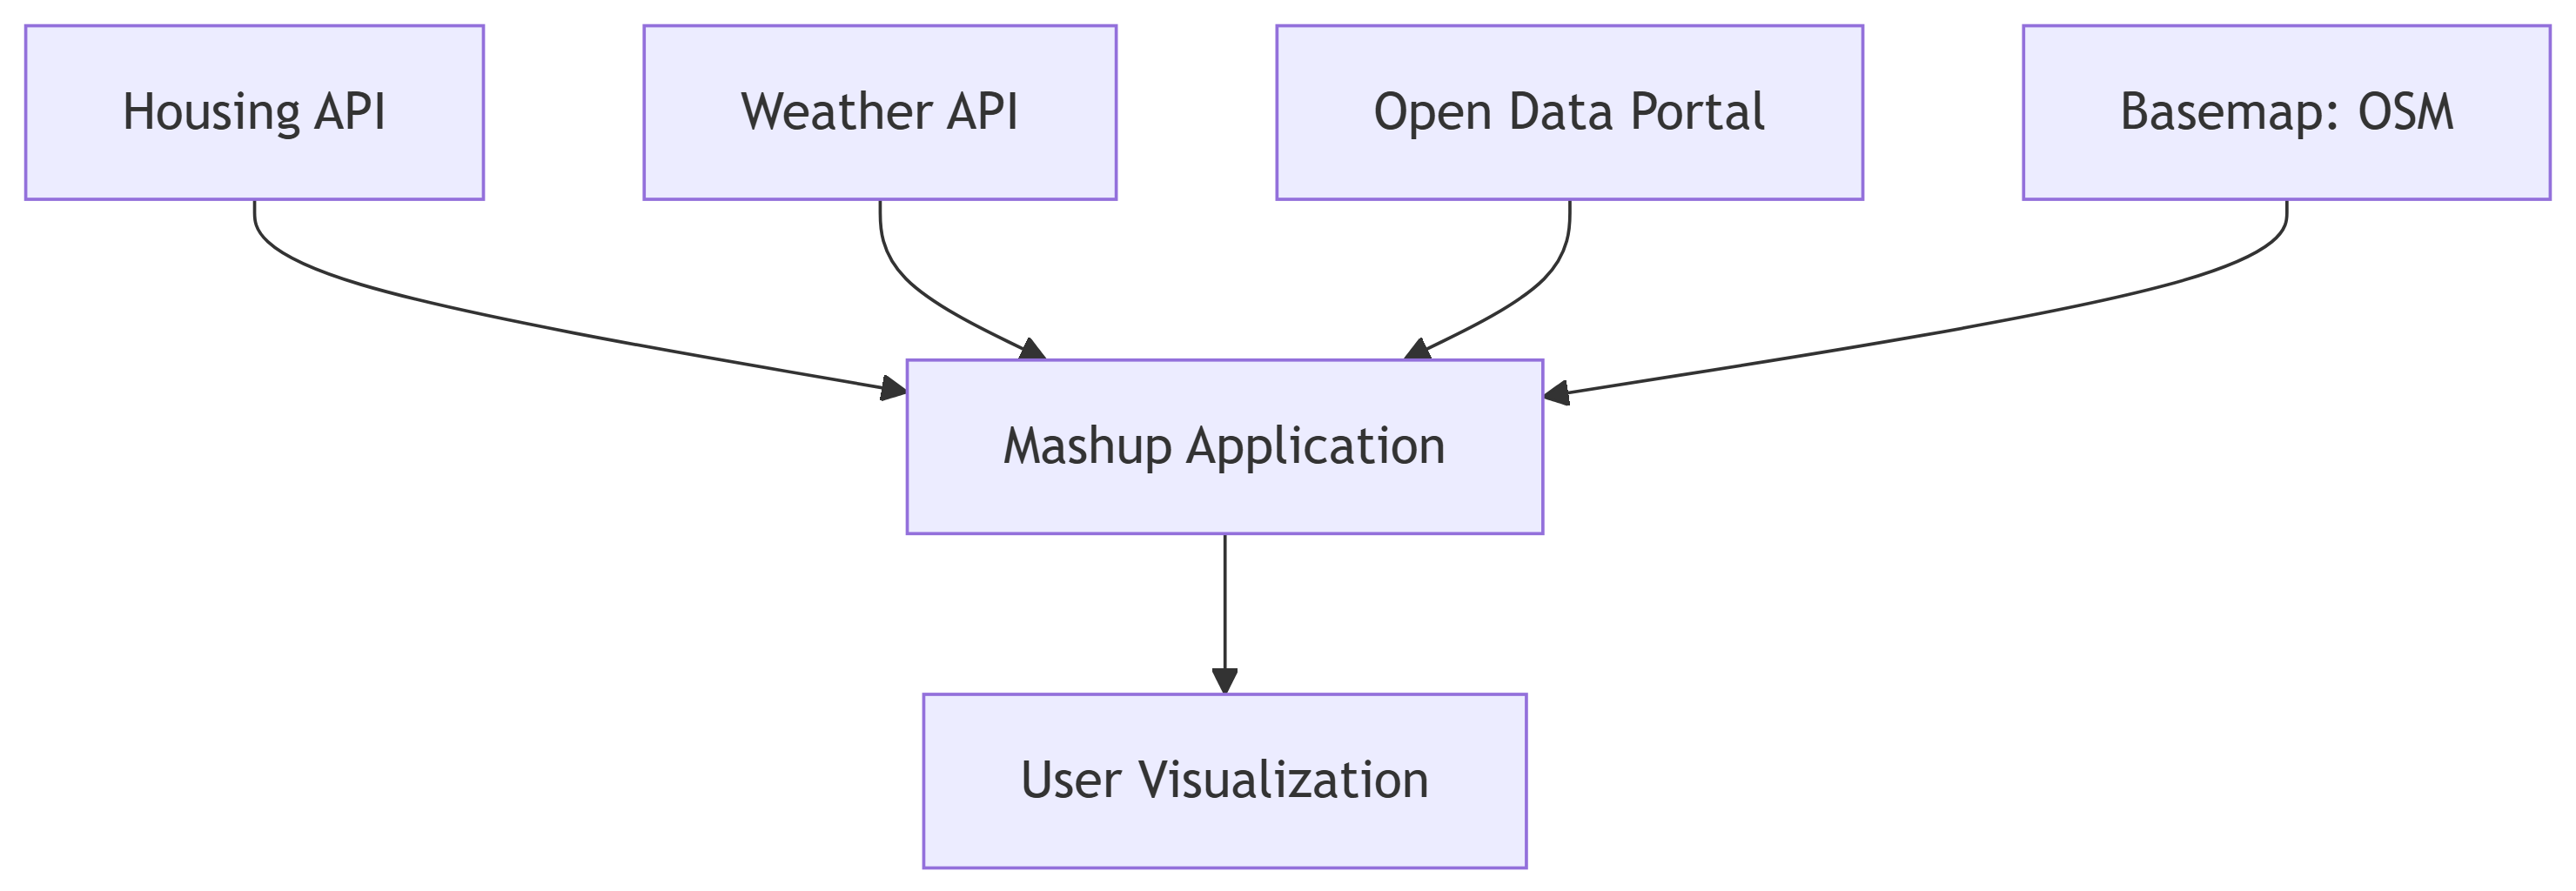
\includegraphics[width=8.35in,height=2.9in]{chapters/module_5/webgis_tools_and_app_files/figure-latex/mermaid-figure-3.png}

}

\caption{\label{fig-geomashup}Integration of multiple data sources in a
geospatial mashup}

\end{figure}%

\subsection{Case Studies}\label{case-studies}

\begin{itemize}
\tightlist
\item
  \textbf{Housing Maps:} Merged 99acres, MagicBricks and Google Maps.\\
\item
  \textbf{HealthMap:} Aggregates disease alerts for global monitoring.\\
\item
  \textbf{COVID-19 Dashboards:} Real-time pandemic data (e.g., Johns
  Hopkins).
\end{itemize}

\begin{center}\rule{0.5\linewidth}{0.5pt}\end{center}

\section{Example Workflow}\label{example-workflow}

A typical workflow integrates FOSS components seamlessly:

\begin{figure}

\centering{

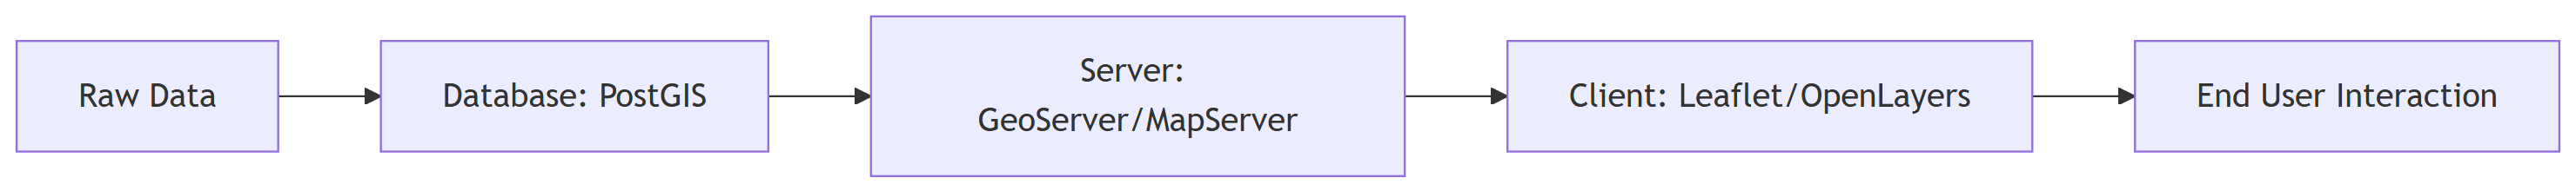
\includegraphics[width=13.07in,height=0.98in]{chapters/module_5/webgis_tools_and_app_files/figure-latex/mermaid-figure-2.png}

}

\caption{\label{fig-foss-workflow}End-to-end workflow of a WebGIS system
with FOSS tools}

\end{figure}%

\begin{center}\rule{0.5\linewidth}{0.5pt}\end{center}

\section{Conclusion}\label{conclusion-9}

This chapter demonstrated how FOSS provides the foundation for WebGIS
development. By integrating server, client, and database tools,
developers can create interoperable systems. Designing applications
requires consideration of scalability, usability, and security. Mashups
illustrate the creativity possible when multiple data sources are
combined. Together, these principles form the foundation of modern
WebGIS applications. The next chapter extends this discussion by
examining Advanced WebGIS and Future Directions. It explores how WebGIS
is evolving beyond 2D maps into domains such as 3D visualization,
real-time streaming, cloud-based systems, and artificial intelligence,
highlighting the trends that will define the next generation of
geospatial technologies.

\chapter{Advanced WebGIS and Future
Directions}\label{advanced-webgis-and-future-directions}

\section{Introduction}\label{introduction-5}

WebGIS has evolved beyond static mapping platforms into advanced systems
supporting 3D visualization, real-time data streaming, and complex
applications across multiple domains. Future trends such as cloud
computing, big data, artificial intelligence (AI), and the semantic web
are transforming how geospatial information is managed and shared. This
chapter provides a comprehensive overview of advanced WebGIS
capabilities, applications, and directions for the future.

\begin{center}\rule{0.5\linewidth}{0.5pt}\end{center}

\section{Advanced Features in WebGIS}\label{advanced-features-in-webgis}

Modern WebGIS platforms extend functionality beyond 2D maps to include
real-time and 3D geospatial visualization.

\subsection{3D Visualization}\label{d-visualization}

With the development of WebGL and libraries like \textbf{CesiumJS}, 3D
visualization has become accessible in web browsers. Applications
include urban planning, terrain modeling, and virtual tourism.

Standards such as \textbf{CityGML} and \textbf{3D Tiles} are critical
for interoperability of 3D geospatial data.

\begin{figure}

\centering{


\includegraphics[width=2.84in,height=2.9in]{chapters/module_5/webgis_trends_files/figure-latex/mermaid-figure-1.png}

}

\caption{\label{fig-3d-visualization}3D visualization in WebGIS using
WebGL and CesiumJS}

\end{figure}%

\subsection{Real-Time Data
Integration}\label{real-time-data-integration}

\begin{itemize}
\tightlist
\item
  \textbf{Traffic Monitoring:} WebGIS platforms stream live traffic
  updates.\\
\item
  \textbf{Weather Dashboards:} Integrate real-time satellite feeds.\\
\item
  \textbf{IoT Networks:} Sensor data (e.g., air quality, water levels)
  integrated directly into WebGIS.
\end{itemize}

\begin{figure}

\centering{

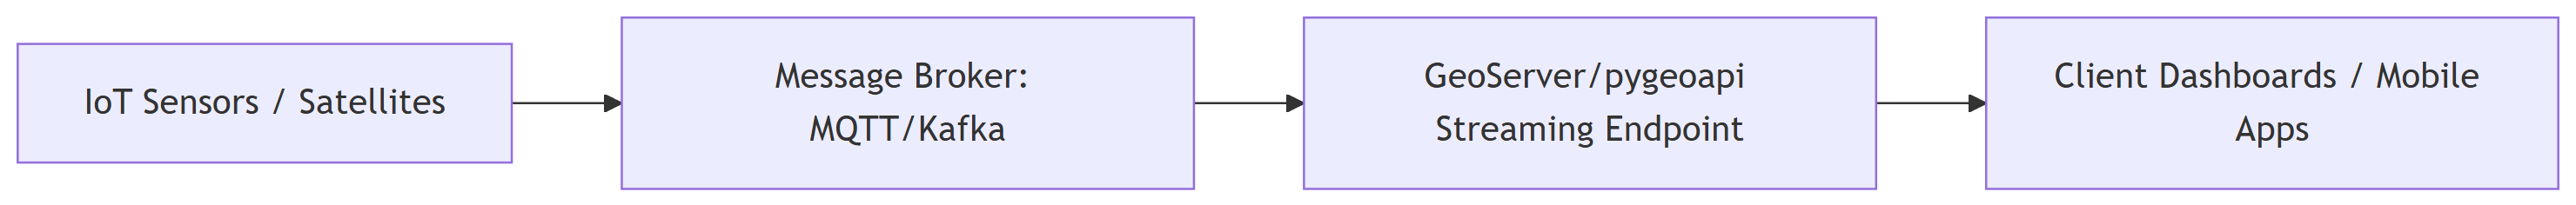
\includegraphics[width=12.19in,height=0.98in]{chapters/module_5/webgis_trends_files/figure-latex/mermaid-figure-5.png}

}

\caption{\label{fig-realtime-arch}Real-time data streaming architecture
in WebGIS}

\end{figure}%

\subsection{Geoportals and SDI}\label{geoportals-and-sdi}

Geoportals act as gateways for sharing geospatial resources across
organizations. Spatial Data Infrastructures (SDI) rely on
interoperability to connect distributed datasets through OGC
standards.\\
Examples include:\\
- \textbf{INSPIRE (European Union)}\\
- \textbf{National Spatial Data Infrastructure (India)}

\begin{center}\rule{0.5\linewidth}{0.5pt}\end{center}

\section{Applications of WebGIS}\label{applications-of-webgis}

WebGIS supports multiple real-world applications across diverse sectors.

\begin{figure}

\centering{

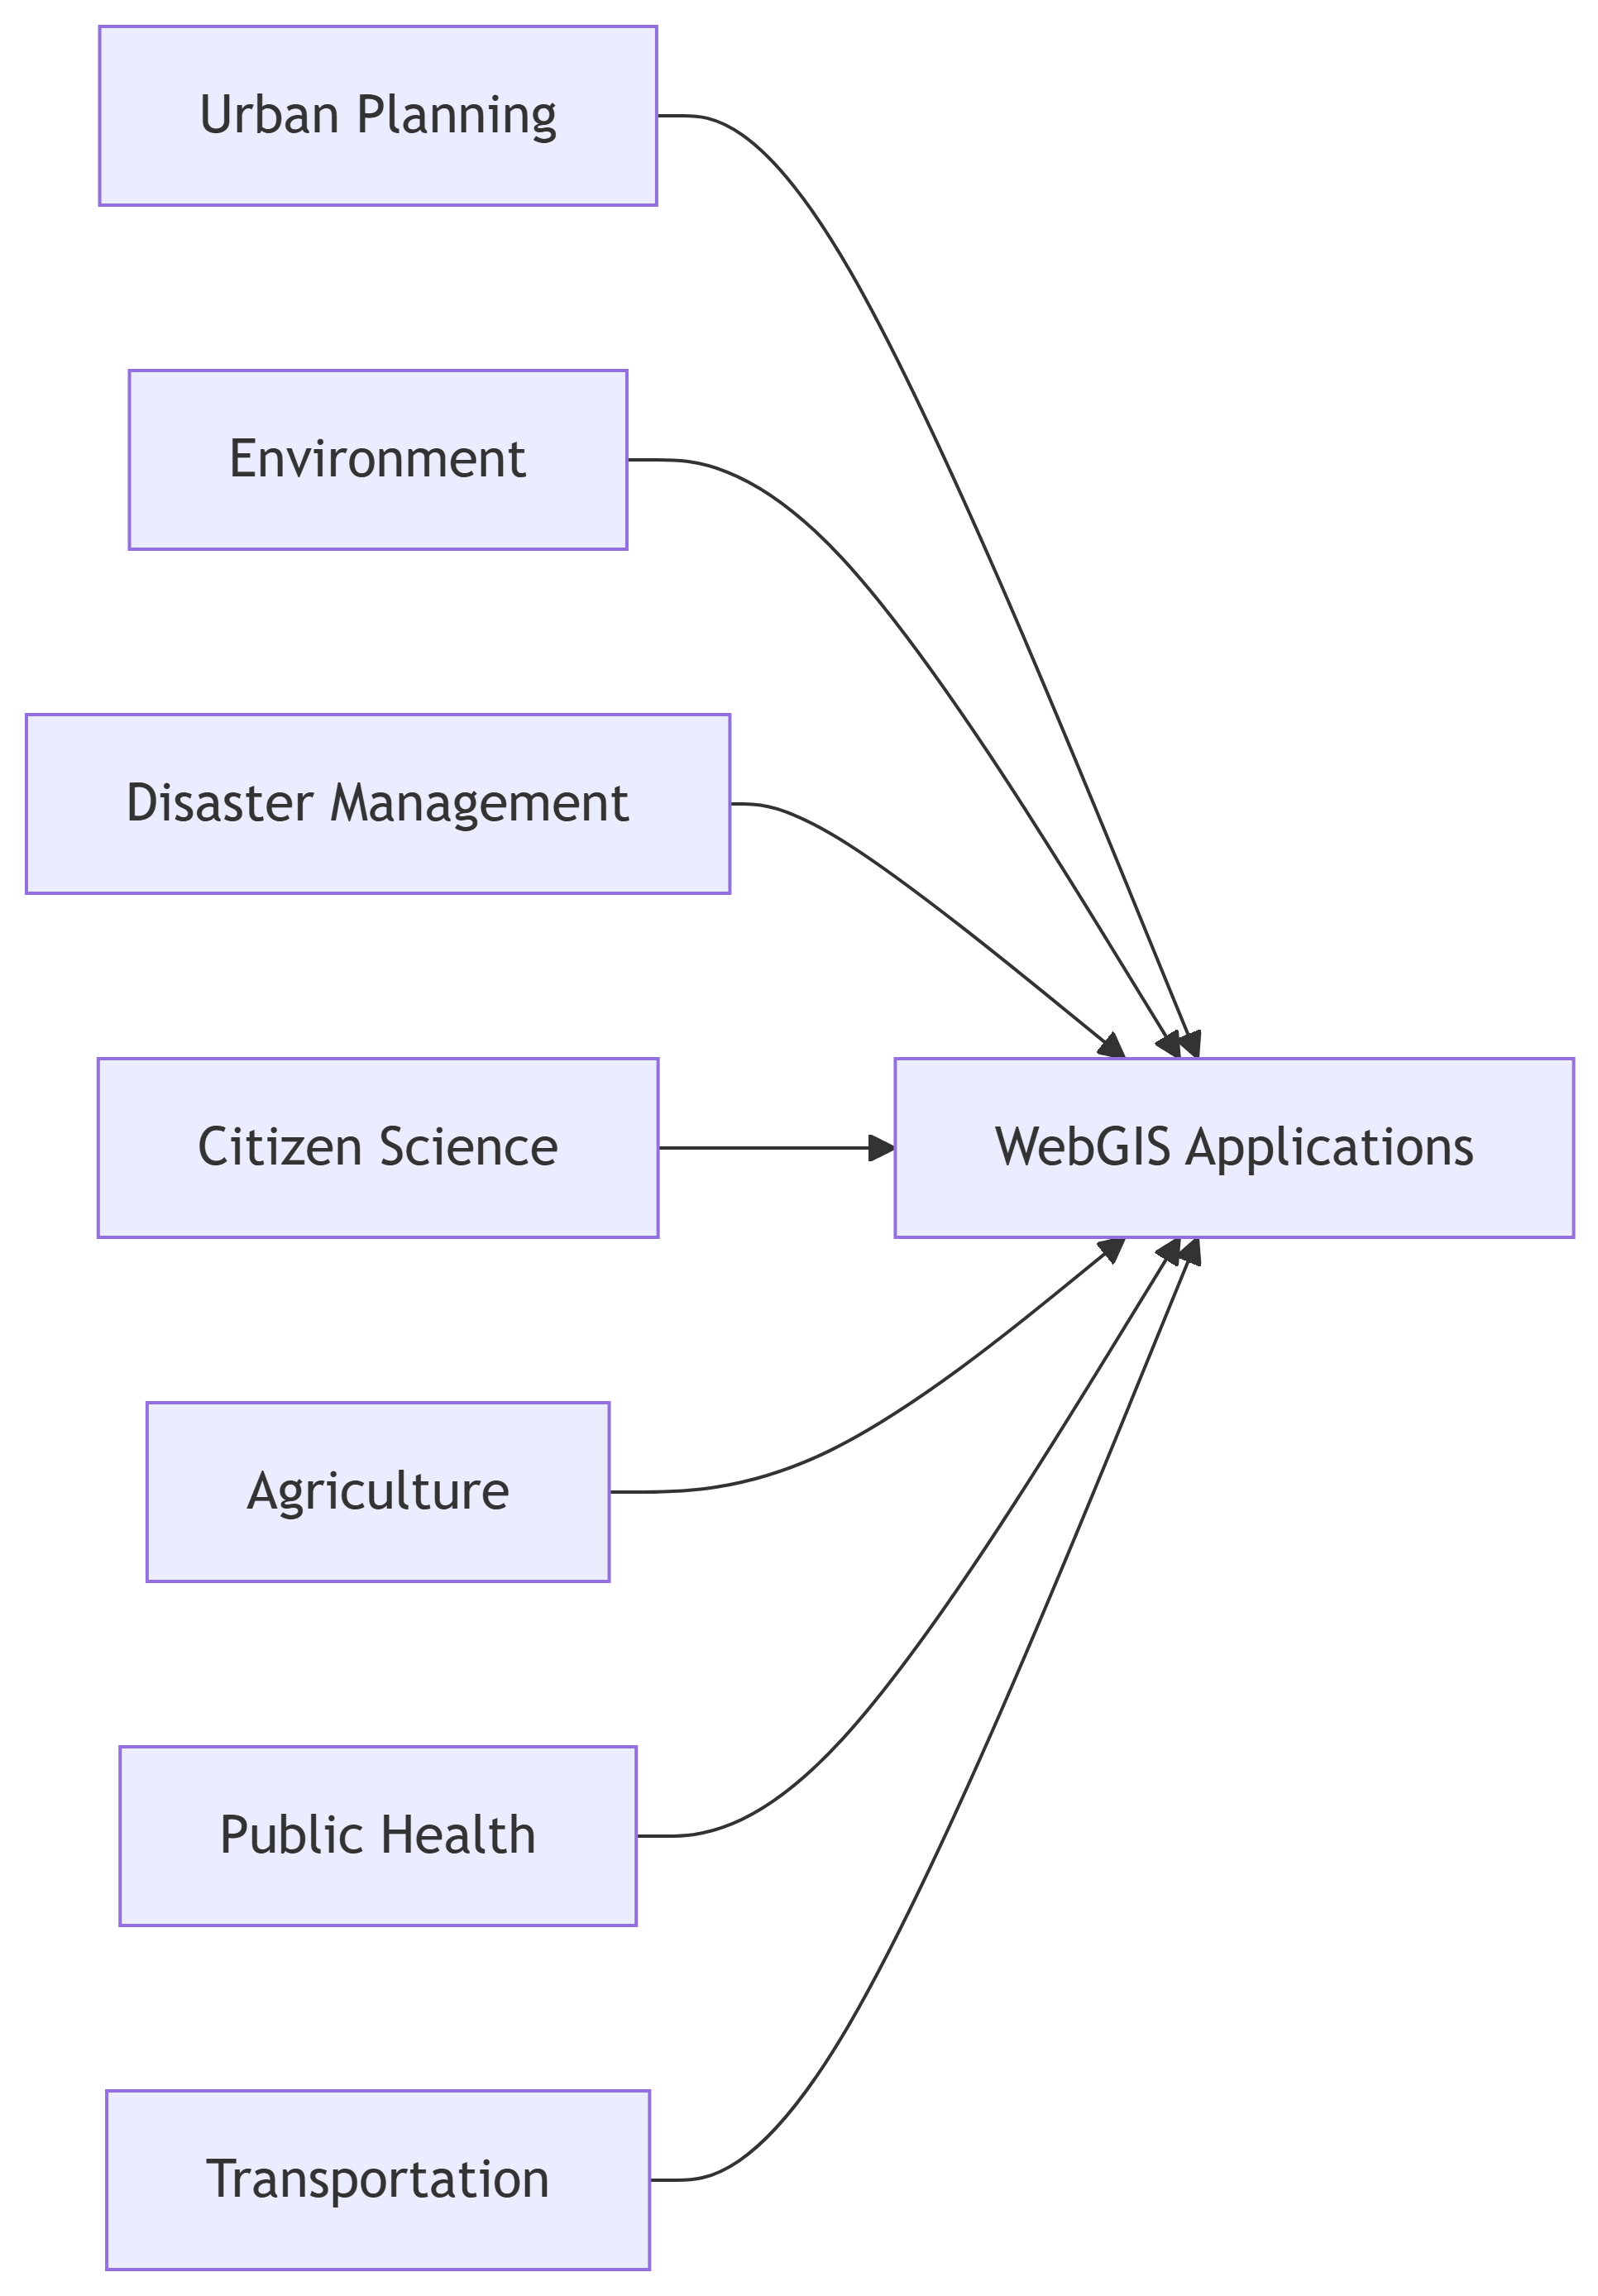
\includegraphics[width=5.04in,height=7.23in]{chapters/module_5/webgis_trends_files/figure-latex/mermaid-figure-4.png}

}

\caption{\label{fig-webgis-applications}Domains of WebGIS applications}

\end{figure}%

\textbf{Table: Applications of WebGIS in Various Domains}

\begin{longtable}[]{@{}
  >{\raggedright\arraybackslash}p{(\linewidth - 4\tabcolsep) * \real{0.2289}}
  >{\raggedright\arraybackslash}p{(\linewidth - 4\tabcolsep) * \real{0.5060}}
  >{\raggedright\arraybackslash}p{(\linewidth - 4\tabcolsep) * \real{0.2651}}@{}}
\toprule\noalign{}
\begin{minipage}[b]{\linewidth}\raggedright
Domain
\end{minipage} & \begin{minipage}[b]{\linewidth}\raggedright
Example Applications
\end{minipage} & \begin{minipage}[b]{\linewidth}\raggedright
Tools Commonly Used
\end{minipage} \\
\midrule\noalign{}
\endhead
\bottomrule\noalign{}
\endlastfoot
Urban Planning & Smart cities, zoning, land management & CesiumJS,
GeoServer \\
Environment & Biodiversity monitoring, air quality & pygeoapi,
OpenLayers \\
Disaster Mgmt & Flood dashboards, wildfire tracking & Leaflet,
GeoNode \\
Agriculture & Crop monitoring, soil analysis & Google Earth Engine,
QGIS \\
Public Health & Disease mapping, COVID-19 dashboards & ArcGIS Online,
Leaflet \\
Transportation & Real-time traffic, smart mobility apps & OpenStreetMap,
GeoServer \\
\end{longtable}

\begin{center}\rule{0.5\linewidth}{0.5pt}\end{center}

\section{Case Studies}\label{case-studies-1}

\begin{enumerate}
\def\labelenumi{\arabic{enumi}.}
\tightlist
\item
  \textbf{COVID-19 Dashboard (Johns Hopkins University):} A global
  WebGIS mashup integrating epidemiological and demographic data using
  ArcGIS Online and REST APIs.\\
\item
  \textbf{OpenAerialMap:} Open imagery catalog enabling disaster
  response through FOSS tools. (
  \href{https://map.openaerialmap.org/}{openaerial})
\item
  \textbf{Humanitarian OpenStreetMap Team (HOT):} Collaborative mapping
  for disaster-prone regions using OSM and tasking managers.
  (\href{https://www.hotosm.org/hubs/}{hotosm})
\end{enumerate}

\begin{center}\rule{0.5\linewidth}{0.5pt}\end{center}

\section{Future Trends in WebGIS}\label{future-trends-in-webgis}

Emerging technologies continue to shape the evolution of WebGIS.

\begin{figure}

\centering{

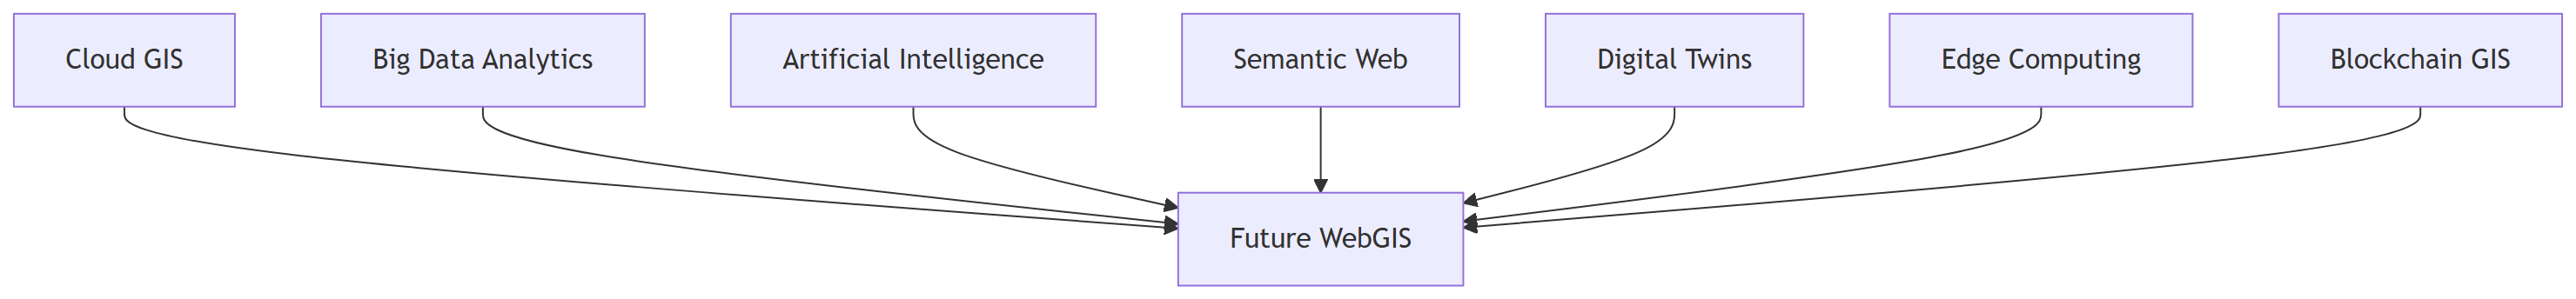
\includegraphics[width=15.58in,height=1.81in]{chapters/module_5/webgis_trends_files/figure-latex/mermaid-figure-3.png}

}

\caption{\label{fig-future-trends}Emerging trends shaping the future of
WebGIS}

\end{figure}%

\subsection{Cloud GIS}\label{cloud-gis}

Cloud GIS leverages distributed computing environments to manage and
analyze large geospatial datasets without the need for local
infrastructure. Platforms such as \textbf{Google Earth Engine (GEE)},
\textbf{ESRI ArcGIS Online}, and \textbf{Amazon Web Services (AWS) Cloud
GIS} provide on-demand scalability. Cloud GIS supports collaborative
workflows, real-time data sharing, and advanced analytics for global
projects.

\begin{itemize}
\tightlist
\item
  \textbf{Advantages:} Scalability, accessibility, and reduced
  infrastructure costs.\\
\item
  \textbf{Challenges:} Data security, reliance on internet connectivity,
  and potential vendor lock-in.\\
\item
  \textbf{Use Case:} GEE supports climate change research by processing
  multi-petabyte satellite archives for land cover change detection.
\end{itemize}

\subsection{Big Geospatial Data}\label{big-geospatial-data}

Big geospatial data refers to high-volume, high-velocity, and
high-variety spatial datasets. These are generated by \textbf{Earth
observation satellites, IoT devices, drones, and crowdsourced platforms}
like OpenStreetMap. Managing these datasets requires \textbf{Hadoop,
Spark, and distributed databases}.

\begin{itemize}
\tightlist
\item
  \textbf{Techniques:} Parallel processing, spatial indexing, and
  distributed storage (HDFS, cloud object storage).\\
\item
  \textbf{Challenges:} Data heterogeneity, integration, and
  visualization at scale.\\
\item
  \textbf{Use Case:} Processing \textbf{Sentinel-2 imagery} streams for
  near real-time agricultural monitoring.
\end{itemize}

\subsection{AI and Machine Learning}\label{ai-and-machine-learning}

Artificial Intelligence and Machine Learning enhance WebGIS by enabling
automated data extraction and predictive analytics. Algorithms in
\textbf{deep learning (CNNs, RNNs)} are widely used in image
classification, change detection, and feature extraction.

\begin{itemize}
\tightlist
\item
  \textbf{Applications:} Land use classification, road detection, flood
  prediction.\\
\item
  \textbf{Advantages:} Improves efficiency and accuracy of geospatial
  analysis.\\
\item
  \textbf{Challenges:} Model bias, training data availability, and
  computational intensity.\\
\item
  \textbf{Use Case:} Using \textbf{TensorFlow with Sentinel-2 data} to
  detect urban expansion patterns.
\end{itemize}

\subsection{Semantic Web}\label{semantic-web}

The Semantic Web improves interoperability by enabling data to be
\textbf{linked, queried, and understood by machines}. In WebGIS, it
allows integration of heterogeneous datasets across domains by adopting
\textbf{Linked Data principles, RDF, and SPARQL queries}.

\begin{itemize}
\tightlist
\item
  \textbf{Applications:} Environmental monitoring portals linking
  climate, biodiversity, and socio-economic datasets.\\
\item
  \textbf{Advantages:} Facilitates discovery and integration of
  geospatial knowledge.\\
\item
  \textbf{Use Case:} \textbf{INSPIRE initiative in Europe} integrates
  environmental datasets across countries using semantic
  interoperability.
\end{itemize}

\subsection{Mobile and Ubiquitous GIS}\label{mobile-and-ubiquitous-gis}

Mobile GIS enables spatial data access, collection, and sharing directly
through smartphones and tablets. Ubiquitous GIS refers to geospatial
access anytime, anywhere.

\begin{itemize}
\tightlist
\item
  \textbf{Applications:} Location-based services (Google Maps, Uber),
  participatory mapping (Mapillary), and disaster response.\\
\item
  \textbf{Advantages:} Enhances citizen engagement, democratizes
  mapping.\\
\item
  \textbf{Challenges:} Accuracy of GPS, data privacy concerns.\\
\item
  \textbf{Use Case:} \textbf{OpenStreetMap (OSM)} field data collection
  apps like \textbf{OSMAnd} and \textbf{MapSwipe} for humanitarian
  mapping.
\end{itemize}

\subsection{Digital Twins}\label{digital-twins}

Digital twins are virtual representations of physical entities,
continuously updated with real-time sensor data. In WebGIS, they
integrate \textbf{IoT, 3D models, and analytics} to simulate and monitor
urban environments.

\begin{itemize}
\tightlist
\item
  \textbf{Applications:} Smart cities, energy management, transportation
  networks.\\
\item
  \textbf{Advantages:} Improves planning, predictive maintenance, and
  decision support.\\
\item
  \textbf{Use Case:} \textbf{Virtual Singapore} project integrates 3D
  GIS and real-time IoT data for urban simulations.
\end{itemize}

\begin{figure}

\centering{


\includegraphics[width=2.88in,height=5.31in]{chapters/module_5/webgis_trends_files/figure-latex/mermaid-figure-2.png}

}

\caption{\label{fig-digital-twin}Future integration of Digital Twins in
WebGIS}

\end{figure}%

\subsection{Edge Computing}\label{edge-computing}

Edge computing processes geospatial data \textbf{closer to the data
source} (e.g., IoT sensors, drones) rather than relying only on
centralized servers.

\begin{itemize}
\tightlist
\item
  \textbf{Advantages:} Reduces latency, supports real-time
  decision-making, lowers network load.\\
\item
  \textbf{Applications:} Disaster response drones, autonomous vehicle
  navigation, smart agriculture sensors.\\
\item
  \textbf{Use Case:} Edge-based flood monitoring systems that trigger
  local alarms before uploading aggregated data to cloud GIS.
\end{itemize}

\subsection{Blockchain in GIS}\label{blockchain-in-gis}

Blockchain introduces \textbf{secure, decentralized, and tamper-proof
records} for geospatial transactions. It ensures \textbf{data
provenance, integrity, and trust} when sharing sensitive geospatial
information.

\begin{itemize}
\tightlist
\item
  \textbf{Applications:} Land registry systems, crowdsourced mapping
  validation, and secure spatial data marketplaces.\\
\item
  \textbf{Advantages:} Transparency, immutability, trust in data-sharing
  ecosystems.\\
\item
  \textbf{Use Case:} \textbf{Blockchain-based land registries} piloted
  in Georgia and Ghana to reduce corruption in property records.
\end{itemize}

\begin{center}\rule{0.5\linewidth}{0.5pt}\end{center}

\section{Conclusion}\label{conclusion-10}

WebGIS has evolved into a sophisticated ecosystem supporting 3D
visualization, real-time integration, and large-scale applications
across domains such as urban planning, disaster response, and citizen
science. Future directions point towards cloud computing, big data
analytics, AI, semantic web, digital twins, edge computing, and
blockchain. These advances will make WebGIS more scalable, intelligent,
and collaborative, playing a key role in addressing global challenges.

\phantomsection\label{refs}
\begin{CSLReferences}{1}{0}
\bibitem[\citeproctext]{ref-albrecht2007}
Albrecht, J. (2007). \emph{Key concepts and techniques in GIS}. London:
SAGE Publications.

\bibitem[\citeproctext]{ref-brimicombe2010}
Brimicombe, A. (2010). \emph{GIS, environmental modeling and
engineering} (2nd ed.). Boca Raton: CRC Press.

\bibitem[\citeproctext]{ref-campbell2011}
Campbell, J. B., \& Wynne, R. H. (2011). \emph{Introduction to remote
sensing} (5th ed.). New York: Guilford Press.

\bibitem[\citeproctext]{ref-saga2008}
Conrad, O., Bechtel, B., Bock, M., Dietrich, H., Fischer, E., Gerlitz,
L., \ldots{} Böhner, J. (2008). System for automated geoscientific
analyses (SAGA) v. 2.0. \emph{Hamburger Beiträge Zur Physischen
Geographie Und Landschaftsökologie}, \emph{19}, 7--12.

\bibitem[\citeproctext]{ref-gdal2023}
GDAL/OGR contributors. (2023). \emph{GDAL/OGR geospatial data
abstraction library}. Retrieved from \url{https://gdal.org}

\bibitem[\citeproctext]{ref-geoserver2024}
GeoServer Development Team. (2024). \emph{GeoServer: An open source
server for sharing geospatial data}. Retrieved from
\url{https://geoserver.org}

\bibitem[\citeproctext]{ref-goodchild2007}
Goodchild, M. F. (2007). \emph{Citizens as sensors: The world of
volunteered geography} (Vol. 69, pp. 211--221).
\url{https://doi.org/10.1007/s10708-007-9111-y}

\bibitem[\citeproctext]{ref-Huisman2009}
Huisman O., de B. R. A. (2009). \emph{Principles of geographic
information systems}. Enschede: ITC.

\bibitem[\citeproctext]{ref-jones2008webgis}
Jones, C. B., \& Purves, R. S. (2008). Web-based geographic information
systems. In J. P. Wilson \& A. S. Fotheringham (Eds.), \emph{Handbook of
geographic information science} (pp. 559--580). Oxford, UK: Blackwell
Publishing.

\bibitem[\citeproctext]{ref-li2020}
Li, S., Dragicevic, S., \& Veenendaal, B. (2020). Advances in geospatial
information science: Mapping the big data challenge. \emph{International
Journal of Digital Earth}, \emph{13}(2), 123--135.
\url{https://doi.org/10.1080/17538947.2019.1651042}

\bibitem[\citeproctext]{ref-mitchell2005webmapping}
Mitchell, T. (2005). \emph{Web mapping illustrated: Using open source
GIS toolkits}. Sebastopol, CA: O'Reilly Media.

\bibitem[\citeproctext]{ref-ogc2025}
OGC. (2025). \emph{OGC standards and resources}. Retrieved from
\url{https://www.ogc.org/standards/}

\bibitem[\citeproctext]{ref-postgis2023}
PostGIS Project Steering Committee. (2023). \emph{PostGIS: Spatial and
geographic objects for PostgreSQL}. Retrieved from
\url{https://postgis.net}

\bibitem[\citeproctext]{ref-qgis2024}
QGIS Development Team. (2024). \emph{QGIS geographic information
system}. Retrieved from \url{https://qgis.org}

\bibitem[\citeproctext]{ref-richards2013}
Richards, J. A. (2013). \emph{Remote sensing digital image analysis: An
introduction} (5th ed.). Berlin: Springer.
\url{https://doi.org/10.1007/978-3-642-30062-2}

\bibitem[\citeproctext]{ref-wilson2008}
Wilson, J. P., \& Fotheringham, A. S. (Eds.). (2008). \emph{The handbook
of geographic information science}. Oxford: Blackwell Publishing.

\bibitem[\citeproctext]{ref-yang2011}
Yang, C., Wong, D., Miao, Q., \& Yang, R. (Eds.). (2011). \emph{Advanced
geoinformation science}. Boca Raton: CRC Press.

\end{CSLReferences}


\backmatter


\end{document}
